\cotefile{152}
\scanpage{1}
\begin{minipage}{0.55\linewidth}
{\Huge\bfseries IMAG}\par
INSTITUT MONTPELLIERAIN\par
ALEXANDER GROTHENDIECK
\end{minipage}\hfill
\begin{minipage}{0.43\linewidth}
\figure{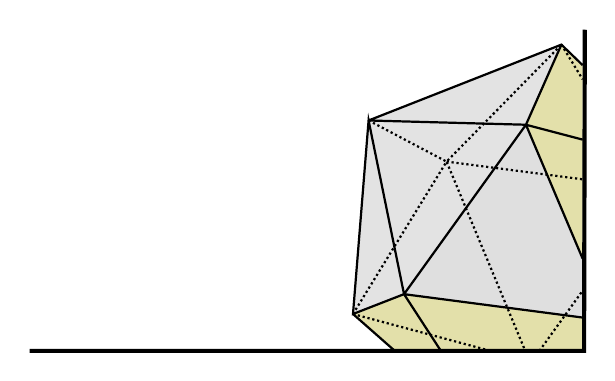
\begin{tikzpicture}[x=0.009cm,y=-0.009cm]
\fill[gray!22] (28,110)--(300,3)--(250,116)--(78,355)--(6,383)--cycle;
\fill[gray!25] (78,355)--(250,116)--(330,137)--(330,310)--(330,435)--(130,435)--cycle;
\fill[olive!25] (300,3)--(330,32)--(330,305)--(250,116)--cycle;
\fill[olive!25] (6,383)--(78,355)--(330,388)--(330,435)--(65,435)--cycle;
\draw[thick] (28,110)--(300,3)--(330,32) (28,110)--(250,116)--(300,3) (250,116)--(330,137) (250,116)--(330,305) (250,116)--(78,355)--(6,383)--(28,110)--(78,355)--(130,435) (78,355)--(330,388) (6,383)--(65,435);
\draw[densely dotted,thick] (28,110)--(138,168)--(300,3) (138,168)--(330,193) (6,383)--(138,168)--(249,435) (6,383)--(200,435) (269,435)--(330,350) (300,3)--(330,52);
\draw[line width=1.5pt] (-450,435)--(332,435)--(333,-18);
\end{tikzpicture}}
\end{minipage}

\scanpage{2}
\figure{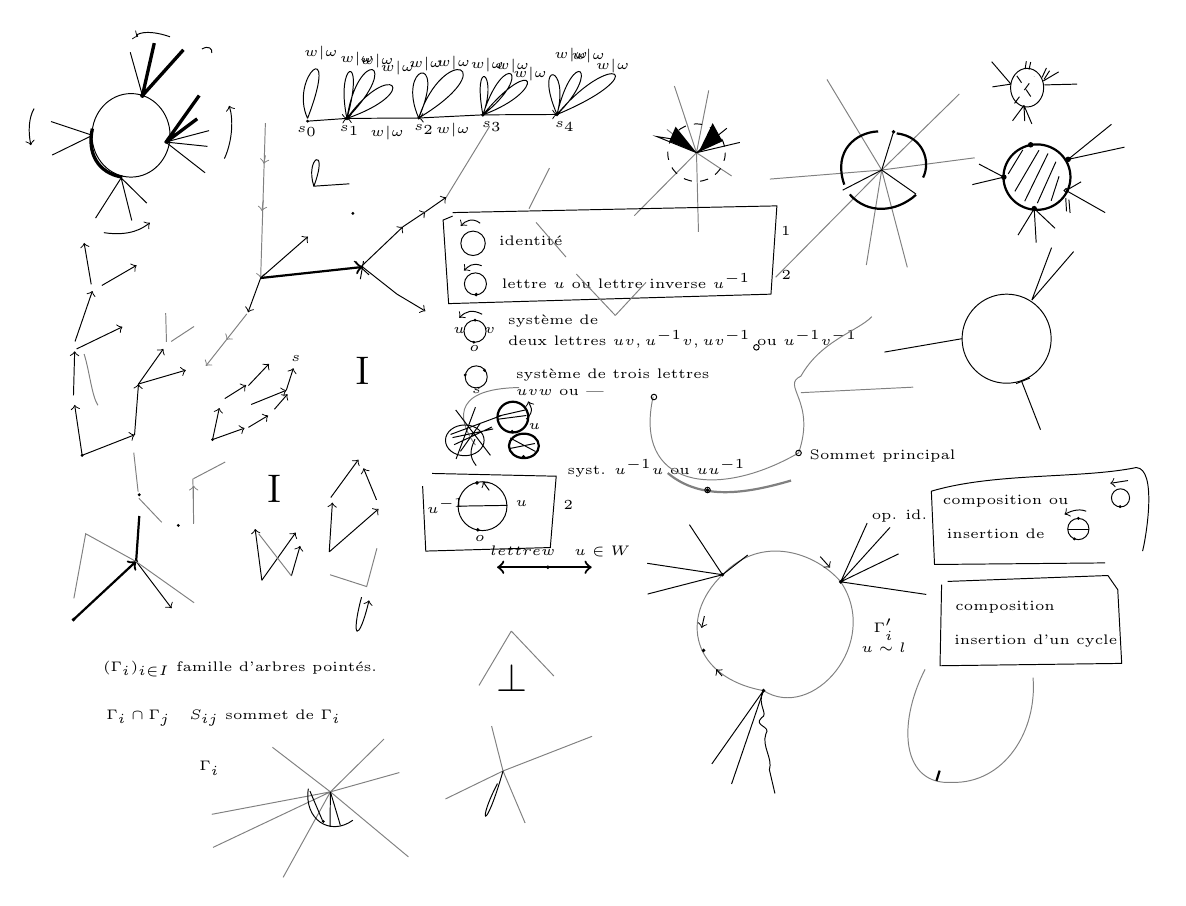
\begin{tikzpicture}[x=.005cm,y=-.005cm,line width=.35pt,every node/.style={font=\tiny,inner sep=1pt}]
\draw (390,295) ellipse (99 and 106);
\draw[very thick] (292,278) .. controls (278,340) and (306,391) .. (368,401) (419,194)--(449,61) (419,194)--(523,78) (479,312)--(563,194) (479,312)--(558,253);
\draw (419,194)--(388,84) (292,295)--(187,260) (292,295)--(190,345) (478,312)--(588,283) (478,312)--(584,323) (478,312)--(578,390) (365,403)--(300,505) (365,403)--(392,511) (365,403)--(430,467);
\fill (419,194) circle(6) (479,312) circle(5);
\draw[->] (489,45) .. controls (428,23) and (398,40) .. (408,44);
\draw[->] (144,227) .. controls (130,251) and (129,287) .. (136,320);
\draw[->] (321,542) .. controls (390,552) and (420,530) .. (438,517);
\draw[->] (627,354) .. controls (649,306) and (649,250) .. (639,220);
\draw (570,76) .. controls (587,66) and (597,75) .. (595,86);
\fill (838,259) circle(4) (938,252) circle(5) (1120,251) circle(4) (1283,243) circle(5) (1471,242) circle(5);
\draw[->] (838,259)--(938,252); \draw[->] (1120,251)--(938,252); \draw[->] (1283,243)--(1120,251); \draw[->] (1283,243)--(1471,242);
\draw (838,252) .. controls (790,147) and (923,31) .. (838,252);
\draw (938,252) .. controls (907,109) and (987,78) .. (938,252) .. controls (965,71) and (1083,103) .. (938,252) .. controls (1048,99) and (1133,184) .. (938,252);
\draw (1120,251) .. controls (1062,118) and (1194,80) .. (1120,251) .. controls (1184,58) and (1339,119) .. (1120,251);
\draw (1283,243) .. controls (1255,94) and (1323,134) .. (1283,243) .. controls (1336,74) and (1419,135) .. (1283,243) .. controls (1416,81) and (1451,181) .. (1283,243);
\draw (1471,242) .. controls (1410,100) and (1505,115) .. (1471,242) .. controls (1512,68) and (1587,128) .. (1471,242) .. controls (1613,73) and (1718,139) .. (1471,242);
\foreach \x/\y in {872/85,963/102,1014/107,1066/125,1138/115,1208/111,1294/116,1358/118,1403/140,1507/92,1550/95,1612/118,1040/289,1207/282}{\node at (\x,\y) {$\unsure{w|\omega}$};}
\foreach \x/\y/\t in {837/286/0,945/282/1,1134/281/2,1306/272/3,1491/273/4}{\node at (\x,\y) {$s_{\t}$};}
\draw (854,424) .. controls (830,351) and (894,318) .. (854,424)--(944,418); \fill (953,493) circle(4);
\draw[gray] (1769,170)--(1825,339)--(1830,540) (1856,181)--(1825,339)--(1667,499) (1825,339)--(1750,280) (1825,339)--(1914,398);
\draw[dashed] (1825,339) circle(73);
\fill (1825,339)--(1772,273)--(1756,310)--cycle;
\fill (1830,338)--(1866,264)--(1891,310)--cycle;
\draw (1825,339)--(1724,298)--(1775,306) (1825,339)--(1902,277) (1825,339)--(1935,313);
\draw[gray] (2156,153)--(2295,383)--(2256,624) (2295,383)--(2492,190) (2295,383)--(2531,352) (2295,383)--(2360,630) (2295,383)--(2026,655) (2295,383)--(2011,406);
\draw[thick] (2200,420) .. controls (2170,333) and (2231,287) .. (2286,285) (2333,290) .. controls (2402,298) and (2420,363) .. (2400,402) (2214,445) .. controls (2259,496) and (2331,491) .. (2382,446);
\draw (2196,434)--(2295,383)--(2382,444) (2295,383)--(2325,286);\fill (2325,286) circle(5);
\draw (2664,174) ellipse(42 and 49);
\draw (2623,165)--(2574,108) (2623,165)--(2576,172) (2659,126)--(2662,107) (2669,128)--(2673,109) (2705,157)--(2744,134) (2708,167)--(2791,165) (2656,219)--(2627,258) (2656,219)--(2676,266) (2656,219)--(2658,259);
\draw[dashed] (2638,144)--(2683,211) (2632,214)--(2682,146);
\draw (2702,148)--(2713,124) (2707,153)--(2721,131);
\draw[thick] (2689,401) ellipse(85 and 83);
\foreach \x/\y in {2605/401,2673/319,2768/356,2682/481}{\fill (\x,\y) circle(7);}
\draw (2605,401)--(2542,368) (2605,401)--(2525,420) (2768,356)--(2878,267) (2768,356)--(2911,325) (2763,435)--(2801,413) (2763,435)--(2862,491) (2682,481)--(2641,548) (2682,481)--(2687,567) (2682,481)--(2735,531) (2762,454)--(2764,488) (2770,458)--(2773,492);
\draw (2763,435) circle(5);\foreach \a/\b/\c/\d in {2616/393/2653/332,2633/437/2694/333,2658/462/2717/341,2690/467/2737/362,2725/461/2745/399}{\draw (\a,\b)--(\c,\d);}
\draw[gray,->] (731,264)--(719,657);\draw[gray,->] (731,346)--(727,367);\draw[gray,->] (726,460)--(722,487);
\draw[thick,->] (719,657)--(978,629);\draw[->] (719,657)--(839,552);\draw[->] (719,657)--(687,744);\draw[gray,->] (684,748)--(632,814);\draw[gray,->] (632,814)--(580,880);
\draw[->] (975,627)--(1080,527);\draw[->] (1080,527)--(1137,489);\draw[->] (1137,489)--(1190,452);\draw[gray] (1190,452)--(1300,272);\draw[->] (975,627)--(1065,698)--(1137,741);\draw (956,614)--(994,649) (980,614)--(972,660);
\draw[->] (289,673)--(271,568);\draw[->] (316,676)--(404,625);
\draw[->] (248,818)--(292,690);\draw[->] (252,837)--(368,781);\draw[gray] (480,819)--(478,746) (492,818)--(550,780);
\fill (266,1107) circle(4);\draw[->] (266,1107)--(247,979);\draw[->] (244,955)--(247,843);\draw[->] (266,1107)--(399,1055);\draw[->] (399,1055)--(409,926);\draw[->] (409,926)--(472,837);\draw[->] (409,926)--(529,891);
\draw[gray] (271,850) .. controls (285,894) and (290,955) .. (306,980);
\fill (597,1067) circle(4);\draw[->] (597,1067)--(614,987);\draw[->] (597,1067)--(678,1038);\draw[->] (628,963)--(682,929);\draw[->] (688,930)--(740,875);\draw[->] (695,978)--(784,942);\draw[->] (784,942)--(802,886);\draw[->] (754,990)--(787,952);\node at (808,862) {$\unsure{s}$};\draw[->] (688,1036)--(738,1006);
\node at (977,893) {\Large $\mathrm I$};\node at (753,1191) {\Large $\mathrm I$};
\fill (411,1207) circle(4) (510,1285) circle(4);\draw[gray] (408,1199)--(397,1100) (410,1216)--(468,1277) (547,1166)--(549,1280) (549,1166)--(629,1124);\draw[gray,->] (549,1280)--(549,1184);
\fill (244,1524) circle(5) (403,1376) circle(5);\draw[thick,->] (244,1524)--(403,1376);\draw[thick] (403,1376)--(411,1261);\draw[->] (403,1376)--(493,1495);\draw[gray] (245,1470)--(275,1306)--(402,1376)--(550,1481);
\draw[->] (722,1424)--(705,1294);\draw[->] (722,1424)--(808,1303);\draw[->] (797,1413)--(819,1337);\draw[gray] (714,1306)--(797,1413);
\draw[->] (897,1214)--(967,1118);\draw[->] (1013,1220)--(980,1140);\draw[->] (893,1352)--(901,1227);\draw[->] (893,1352)--(1018,1243);\draw[gray] (895,1410)--(988,1440)--(1014,1343);\draw[->] (975,1467) .. controls (946,1575) and (968,1585) .. (994,1475);
\draw (1206,491)--(2029,474)--(2014,698)--(1196,722)--(1182,510)--(1206,500);
\draw (1258,569) circle(31);\draw[->] (1276,518)..controls (1256,502) and (1237,513)..(1227,525);\node[anchor=west] at (1316,563) {identité};\node at (2052,539) {$1$};
\draw (1264,672) circle(28);\fill (1266,699) circle(5);\draw[->] (1280,626)..controls (1256,616) and (1246,628)..(1235,638);\node[anchor=west] at (1323,665) {lettre $u$ ou lettre \unsure{inverse} $u^{-1}$};\node at (2053,649) {$2$};
\draw[gray] (1400,481)--(1452,378) (1418,516)--(1494,604) (1619,752)--(1520,647) (1619,752)--(1697,668);
\draw (1263,792) circle(28);\fill (1263,764) circle(4) (1260,820) circle(4);\draw[->] (1281,749)..controls (1256,736) and (1240,741)..(1223,758);\node at (1223,790) {$u$};\node at (1301,790) {$v$};\node at (1261,836) {$o$};
\node[anchor=west,align=left] at (1339,793) {système de\\deux lettres $uv,u^{-1}v,uv^{-1}$ ou $u^{-1}v^{-1}$};
\draw (1266,908) circle(28);\fill (1238,903) circle(4) (1287,891) circle(4);\node at (1267,943) {$\unsure{s}$};\node[anchor=west,align=left] at (1359,921) {système de trois lettres\\$\unsure{uvw}$ ou \unsure{---}};
\draw[gray] (1375,935) .. controls (1190,938) and (1227,1030)..(1264,1081);
\draw[thick] (1359,1010) circle(39) (1387,1083) ellipse(38 and 31);\draw (1324,1015)--(1393,1006) (1324,1007)--(1390,992) (1352,1063)--(1416,1097) (1350,1090)--(1415,1077);\fill (1357,1047) circle(5) (1386,1111) circle(5);\node at (1414,1035) {$u$};\draw[->] (1393,1015)..controls(1417,993)and(1401,979)..(1398,970);
\draw (1237,1069) ellipse(49 and 39);\draw (1214,992)--(1302,1107) (1264,985)--(1215,1116) (1201,1054)--(1330,1006) (1206,1062)--(1309,1040) (1210,1080)--(1306,1035) (1226,1097)--(1277,1025) (1263,1066) .. controls (1250,1093) and (1248,1111)..(1266,1133);
\draw (1130,1185)--(1138,1350)--(1454,1341)--(1469,1160)--(1154,1153);
\draw (1282,1236) circle(62);\draw (1219,1236)--(1345,1234);\fill (1270,1296) circle(5) (1268,1177) circle(5);\node at (1275,1318) {$o$};\node at (1381,1230) {$u$};\node at (1189,1235) {$u^{-1}$};\node at (1500,1234) {$2$};\draw[->] (1299,1196)--(1283,1174);\node[anchor=west] at (1490,1140) {syst. $u^{-1}u$ ou $uu^{-1}$};
\node at (1480,1350) {$\unsure{\text{lettre }w}\quad u\in W$};\draw[<->,thick] (1319,1391)--(1559,1391);\fill (1448,1391) circle(5);
\draw[gray] (1715,958)..controls(1664,1187)and(1874,1222)..(2084,1101)..controls(2130,969)and(2038,930)..(2090,906);\draw[gray] (2090,906)..controls(2141,815)and(2235,792)..(2270,755) (2090,948)--(2375,934);\draw[gray,thick] (1752,1152)..controls(1837,1223)and(1952,1204)..(2065,1171);
\foreach \x/\y in {1717/959,1977/833,2084/1101,1853/1195}{\draw (\x,\y) circle(7);}\fill (1853,1195) circle(5);
\node[anchor=west] at (2104,1108) {\unsure{Sommet} \unsure{principal}};
\draw (2612,811) circle(113);\draw (2499,811)--(2302,845) (2676,713)--(2726,580) (2676,713)--(2782,590) (2650,919)--(2698,1042);\draw (2636,925)--(2671,911);
\draw[gray] (1891,1410)..controls(1777,1520)and(1816,1672)..(1995,1704)..controls(2120,1784)and(2295,1583)..(2191,1428)..controls(2129,1355)and(1991,1305)..(1891,1410);
\foreach \x/\y in {1891/1410,1843/1602,1995/1704,2191/1428}{\fill (\x,\y) circle(5);}
\draw (1891,1410)--(1700,1381) (1891,1410)--(1701,1459) (1891,1410)--(1807,1283) (1891,1410)--(1955,1360) (2191,1428)--(2258,1279) (2191,1428)--(2316,1290) (2191,1428)--(2338,1357) (2191,1428)--(2408,1460) (1995,1704)--(1864,1890) (1995,1704)--(1914,1941);
\draw (1995,1704)..controls(1976,1739)and(2010,1764)..(1990,1773)..controls(1968,1794)and(2016,1794)..(2001,1814)..controls(1990,1846)and(2019,1875)..(2010,1905)--(2024,1965);\draw[->] (1845,1515)--(1838,1545);\draw[->] (1890,1667)--(1875,1650);\draw[->] (2139,1364)--(2164,1392);
\node at (2340,1260) {\uline{\unsure{op. id.}}};\node[align=center] at (2300,1565) {$\unsure{\Gamma'_i}$\\$\unsure{u\sim l}$};
\draw (2421,1198)--(2429,1384)--(2862,1380) (2421,1198)..controls(2583,1150)and(2799,1167)..(2941,1138)..controls(2994,1141)and(2967,1310)..(2957,1350);
\node[anchor=west] at (2442,1223) {\uline{composition} ou};\draw (2901,1215) circle(23);\fill (2900,1237) circle(4);\draw[->] (2920,1171)--(2875,1178);
\node[anchor=west] at (2452,1305) {\uline{insertion} de};\draw (2794,1294) circle(27);\draw (2767,1294)--(2821,1294);\fill (2794,1267) circle(4) (2784,1319) circle(4);\draw[->] (2814,1249)..controls(2793,1240)and(2770,1251)..(2759,1257);
\draw (2447,1435)--(2443,1641)--(2904,1635)--(2894,1448)--(2869,1412)--(2462,1427);
\node[anchor=west] at (2474,1492) {composition};\node[anchor=west] at (2471,1579) {insertion d'un cycle};
\draw[gray] (2405,1650)..controls(2332,1793)and(2348,1944)..(2472,1937)..controls(2606,1941)and(2690,1807)..(2679,1671);\draw[thick] (2442,1907)--(2434,1933);
\node[anchor=west] at (311,1649) {$(\Gamma_i)_{i\in I}$ famille \unsure{d'arbres} \unsure{pointés}.};
\node[anchor=west] at (319,1773) {$\Gamma_i\cap\Gamma_j\quad S_{ij}$ sommet de $\Gamma_i$};\node at (589,1901) {$\Gamma_i$};
\draw[gray] (896,1961)--(749,1848) (896,1961)--(1032,1827) (896,1961)--(1094,2126) (896,1961)--(776,2178) (896,1961)--(598,2102) (896,1961)--(595,2018) (896,1961)--(1071,1912);
\draw (840,1953)..controls(828,2031)and(895,2075)..(953,2033) (844,1959)--(876,2034) (896,1961)--(895,2050) (896,1961)--(921,2045);\fill (878,2036) circle(4);
\draw[gray] (1334,1908)--(1305,1794) (1334,1908)--(1188,1979) (1334,1908)--(1560,1820) (1334,1908)--(1390,2040);\draw (1320,1940)..controls(1268,2038)and(1287,2073)..(1334,1908);
\draw[gray] (1355,1553)--(1273,1691) (1355,1553)--(1463,1667);\node at (1356,1672) {\Large $\perp$};
\end{tikzpicture}}
\mspage{1}

\scanpage{3}
\par\noindent\diagram{\begin{tikzcd}[row sep=small]
\text{disques découpés \unsure{avec} origine fixée}\arrow[d,leftrightarrow]\\
\text{\deleted{\unsure{gr.}} arbre circularisé pointé}
\end{tikzcd}}\par

\deleted{\unsure{mots}} type de mots \deleted{\unsure{en}} $=$ \deleted{\unsure{disq}} arbres \inserted{\unsure{plans ou}} pointés, \deleted{\unsure{et coupés}} bouts libres, \uline{en l'origine} \unsure{seult} et \deleted{\unsure{orientés}} \unsure{plats} à l'intérieur

\par\noindent\diagram{\begin{tikzcd}[column sep=small]
\text{disques\inserted{or.}\uline{\unsure{linéarisés}}}\arrow[r,leftrightarrow]&
\text{\deleted{graphes}\inserted{arbres} circularisés}\arrow[r,leftrightarrow]&
\begin{gathered}\text{\unsure{ordres}}\\\text{à involuti.}\\\text{\unsure{sans} pt fixe}\end{gathered}
\end{tikzcd}}\par
\unsure{ou encore}
\par\noindent\diagram{\begin{tikzcd}[column sep=small]
\begin{gathered}\text{disques\inserted{or.}}\\\text{\deleted{\unsure{topologiquement}}}\\\text{découpés,}\end{gathered}\arrow[r,leftrightarrow]&
\begin{gathered}\text{\deleted{graphes}\inserted{arbres}}\\\text{(: bouts libres)}\\\text{circularisés}\end{gathered}\arrow[r,leftrightarrow]&
\begin{gathered}\text{\unsure{ordres}}\\\text{à inv.}\\\text{\unsure{cpt.} \unsure{lin.}}\\\text{sans pt fixe}\\\text{\unsure{mais}}\\\text{\unsure{pointés}.}\end{gathered}
\end{tikzcd}}\par
avec condition que chaque \unsure{cpt.} découpée \unsure{contient} au moins un sommet, ou au plus un sommet (au choix)

\figure{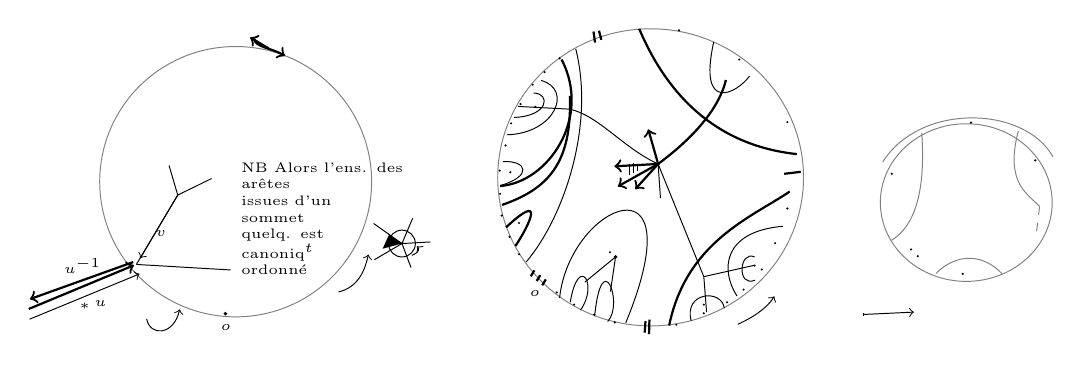
\begin{tikzpicture}[x=.005cm,y=-.005cm,every node/.style={font=\tiny,inner sep=1pt},line width=.35pt]
\draw[gray] (670,640) ellipse(345 and 343);\draw[->,thick] (717,277)..controls(718,299)and(763,301)..(795,321);\draw[->,thick] (754,302)--(707,274);
\draw (418,850)--(523,674)--(501,599) (523,674)--(609,632) (418,850)--(657,864);\draw[->] (523,674)--(428,834);
\draw[->,thick] (410,844)--(148,938);\draw[->,thick] (145,963)--(412,852);\draw[->] (147,989)--(426,874);
\node at (282,853) {$u^{-1}$};\node at (327,950) {$u$};\node at (287,955) {$*$};\node at (480,771) {$v$};
\fill (644,975) circle(5);\node at (645,1011) {$o$};\draw[->] (444,988)..controls(453,1034)and(513,1030)..(528,964);
\node[anchor=west,align=left,text width=2.65cm] at (676,734) {\uline{NB} Alors l'ens. des arêtes\\issues d'un\\sommet\\quelq. est\\canoniq$^{\unsure{t}}$\\\uline{ordonné}};
\draw (1092,797) circle(34);\draw (1092,797)--(1020,746) (1092,797)--(1119,733) (1092,797)--(1164,793) (1092,797)--(1115,858) (1092,797)--(1022,838);\fill (1092,797)--(1059,775)--(1043,810)--cycle;\draw[->] (1117,827)..controls(1139,818)and(1135,809)..(1130,804);\draw[->] (931,920)..controls(983,907)and(998,863)..(1007,825);
\draw[gray] (1723,629) ellipse(388 and 377);
\foreach \x/\y in {1345/726,1341/671,1340/612,1355/548,1369/492,1393/443,1424/394,1454/362,1492/327,1795/256,1948/330,2070/489,2070/708,2039/796,2005/863,1959/914,1917/946,1788/1003,1632/997,1580/977,1529/952,1485/921,1437/887,1389/824,1365/780}{\fill (\x,\y) circle(3);}
\draw[thick] (1578,259)--(1582,287) (1592,257)--(1598,280) (2062,620)--(2104,615) (1710,994)--(1708,1023) (1720,990)--(1719,1027) (1428,865)--(1419,880) (1443,877)--(1434,892) (1457,888)--(1448,903);
\node at (1429,925) {$o$};
\draw (1426,415)..controls(1470,416)and(1465,474)..(1376,477);
\draw (1445,383)..controls(1527,406)and(1480,518)..(1358,521);
\draw[thick] (1497,330)..controls(1574,477)and(1464,642)..(1341,651);
\draw (1533,303)..controls(1582,497)and(1503,731)..(1407,844);
\draw[thick] (1518,422)..controls(1524,592)and(1464,658)..(1346,699);
\draw (1348,589)..controls(1410,586)and(1424,626)..(1341,650);
\draw[thick] (1356,756)..controls(1458,661)and(1415,751)..(1380,803);
\draw (1386,449)--(1518,456)..controls(1591,472)and(1654,555)..(1742,595);
\draw[thick] (1694,252)..controls(1760,408)and(1879,547)..(2094,570);
\draw[thick] (1742,595)..controls(1853,513)and(1901,438)..(1914,382);
\draw (1883,286)..controls(1843,467)and(1941,417)..(1974,372);
\draw (1742,595)--(1858,881)--(1865,971) (1858,881)--(1987,852);
\draw[thick] (1770,1005)..controls(1814,792)and(1980,730)..(2076,665);
\draw (1660,998)..controls(1840,560)and(1517,697)..(1492,935);
\draw (1519,946)..controls(1540,821)and(1592,900)..(1545,966);
\draw (1581,981)..controls(1599,798)and(1656,950)..(1614,995);
\fill (1634,831) circle(5);\draw (1634,831)--(1621,919) (1634,831)--(1556,895);
\draw (1826,993)..controls(1806,920)and(1903,911)..(1910,961);
\draw (2059,753)..controls(1903,767)and(1901,866)..(1942,930);
\draw (1987,831)..controls(1947,813)and(1941,910)..(1988,890);
\draw[->] (1944,1002)..controls(2000,977)and(2026,949)..(2037,931);
\foreach \x/\y in {1430/450,1367/616,1389/745,1620/819,1858/952,1858/974,1987/853}{\fill (\x,\y) circle(3);}
\draw[thick,->] (1742,595)--(1717,507);\draw[thick,->] (1742,595)--(1631,601);\draw[thick,->] (1742,595)--(1640,652);\draw[thick,->] (1742,595)--(1684,659);\draw (1742,595)--(1748,682);\fill (1742,595) circle(5);\draw (1670,594)--(1670,622) (1680,593)--(1680,618) (1690,594)--(1690,614);
\draw[gray] (2524,693) ellipse(218 and 200);\draw[gray] (2312,590)..controls(2407,439)and(2672,447)..(2744,577) (2411,516)..controls(2422,674)and(2389,756)..(2334,789) (2656,512)..controls(2620,647)and(2685,674)..(2710,703) (2447,873)..controls(2503,817)and(2571,826)..(2615,874);
\foreach \x/\y in {2536/490,2335/620,2384/812,2401/829,2515/874,2699/586}{\fill (\x,\y) circle(3);}\draw[gray,dashed] (2710,703)--(2701,779);
\draw[->] (2262,977)--(2391,971);\draw (2263,973)--(2263,980);
\end{tikzpicture}}

\figure{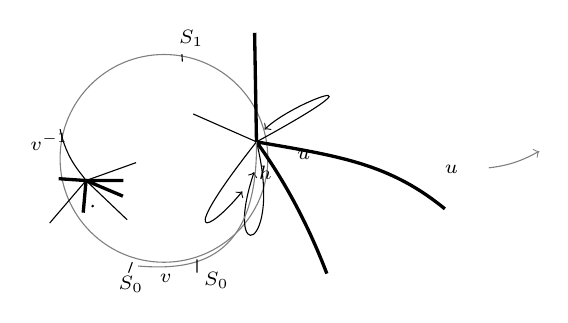
\begin{tikzpicture}[x=.006cm,y=-.006cm,every node/.style={font=\scriptsize,inner sep=1pt}]
\draw[gray] (365,350) ellipse(220 and 220);
\draw (145,288)..controls(159,354)and(189,380)..(200,397);
\fill (200,397) circle(4) (561,315) circle(4);
\draw[very thick] (200,397)--(142,393) (200,397)--(279,397) (200,397)--(278,430) (200,397)--(194,465);
\draw (200,397)--(306,359) (200,397)--(287,480) (200,397)--(123,487);\fill (214,451) circle(3);
\draw (561,315)--(427,256);\draw[very thick] (561,315)--(557,84) (561,315)..controls(733,345)and(842,360)..(960,457) (561,315)..controls(624,402)and(672,495)..(710,594);
\draw[->] (561,315)..controls(862,151)and(639,229)..(578,289);
\draw[->] (561,315)..controls(387,536)and(457,510)..(531,420);
\draw[->] (561,315)..controls(619,548)and(488,582)..(556,379);
\draw[gray] (561,315)..controls(564,567)and(432,588)..(310,578);
\draw (403,129)--(404,145) (298,570)--(290,592) (435,564)--(435,592);
\node at (423,96) {$S_1$};\node at (122,315) {$\unsure{v^{-1}}$};\node at (295,617) {$S_0$};\node at (369,604) {$v$};\node at (476,608) {$S_0$};\node at (661,343) {$u$};\node at (580,380) {$\unsure{h}$};\node at (974,374) {$\unsure{u}$};\draw[gray,->] (1053,370)..controls(1110,364)and(1140,345)..(1160,335);
\end{tikzpicture}}

La cat. des ``\deleted{\unsure{mots}}\inserted{types} de mots'' de long. $n$ équivaut à la cat. isotopique des systèmes \unsure{formés|finis} d'un disque $D$ \inserted{en général orienté} \unsure{d'une|d'un} ``découpage en cordes'' de ce disque, avec au moins un sommet sur chaque \unsure{cpt.} découpée sur $\dot D$ par les extrémités des cordes,
\[
(D,\omega,\deleted{\unsure{K}},\deleted{\unsure{S}},K,S_0)
\]
$D$ le disque top.\par
$\omega$ une orientation de $D$\par
$K\subset D$ le 1-complexe top. (\unsure{réunion} \unsure{top.} de segments) des cordes du découpage\par
$S_0\in S$ \deleted{\unsure{est la composante} \unsure{de} \unsure{l'origine} $(\dot D\setminus K\cap\dot D)$}\par
$S\subset\dot D$, soit $R_0$ l'unique comp. connexe de $D\setminus K$ contenant $S_0$

\[
\uline{\text{\unsure{ordre} réduit}}=\sum_{\alpha\in\pi_0(\dot D\setminus K\cap\dot D)}(\operatorname{Card}(\alpha\cap S)-1)
\]
\[
(\text{pour }\deleted{\unsure{\alpha\in\pi_0}}\ \alpha\subset R_0)
\]
\margin{$v\,u^{-1}u$\par $u\,v\,u^{-1}$}

Type de mot \uline{trivial} : \unsure{ordre} réduit $=0$\par
\uline{Type de mot \unsure{totalitaire}} : $K=\varnothing$\par
(\unsure{non} trivial)

\[
\operatorname{Card}S=n\quad(\ne0)\qquad\text{donc }S\ne\varnothing
\]
\[
\deleted{S\cap S_0\ne\varnothing}\quad
\forall\alpha\in\pi_0(\dot D\setminus K\cap\dot D):
\left\{\begin{array}{l}
S\cap\alpha\ne\varnothing\\
\operatorname{Card}S\cap\alpha=1\quad\text{si }\alpha\not\subset R_0
\end{array}\right.
\]
Type de mot trivial,\par
si $\unsure{2}\ \operatorname{Card}S\cap\alpha$.

\figure{
\begin{tikzpicture}
\node[rotate=180,align=left,font=\ttfamily\scriptsize] { /*JOB=CRAY1,ACCT=\unsure{*********|********},ALL=\unsure{M06|MO6}\\ // JOB MSGLEVEL=(1,1),MSGCLASS=A\\ // EXEC CSSBATCH\\ //CRAYIN DD *};
\node[rotate=180,font=\ttfamily\scriptsize] at (6,0) {\unsure{J0202CNU|JO202CNU}};
\end{tikzpicture}}
\mspage{2}

\scanpage{4}
\figure{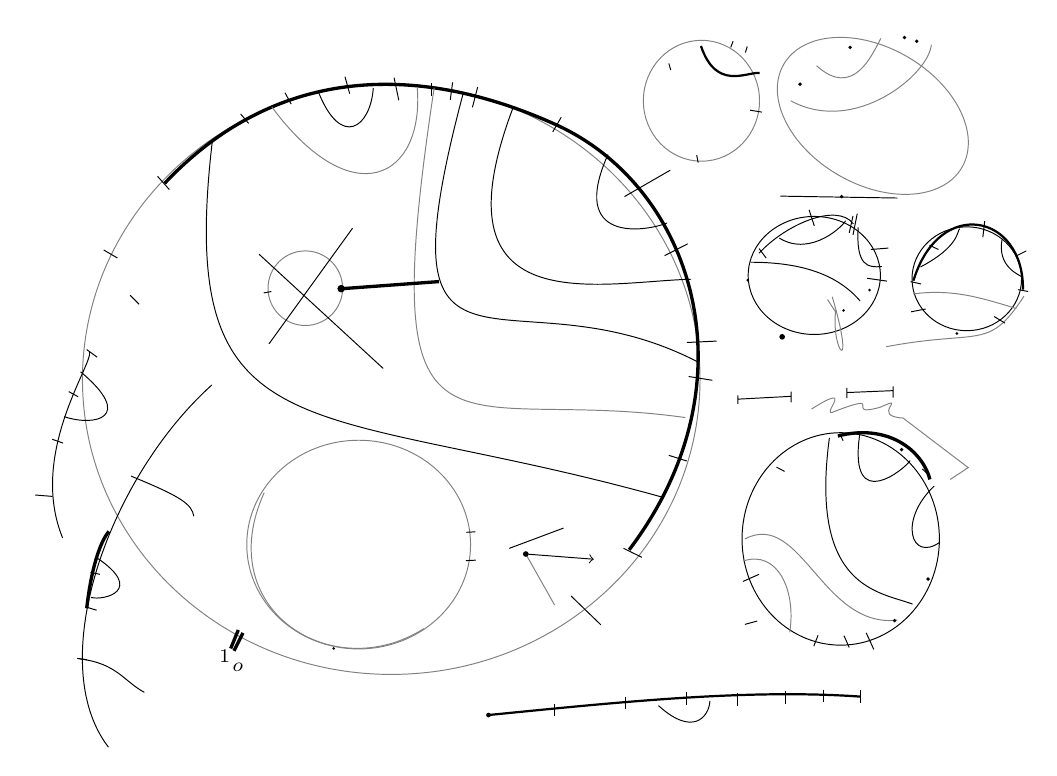
\begin{tikzpicture}[x=.006cm,y=-.006cm,line width=.35pt,every node/.style={font=\scriptsize,inner sep=1pt}]
\draw[gray] (802,865) ellipse(654 and 625);
\draw[very thick] (322,450)..controls(549,209)and(846,186)..(1156,328)..controls(1443,462)and(1574,872)..(1306,1226);
\draw (423,361)..controls(344,1037)and(630,907)..(1374,1114);
\draw[gray] (549,288)..controls(721,520)and(873,438)..(857,246);
\draw (648,257)..controls(696,377)and(758,332)..(764,248);
\draw[gray] (893,247)..controls(763,1108)and(930,876)..(1425,946);
\draw (955,257)..controls(768,960)and(1049,619)..(1453,829);
\draw (1061,287)..controls(885,750)and(1243,658)..(1437,653);
\draw (1261,389)..controls(1177,576)and(1338,553)..(1386,534);
\foreach \x/\y/\a/\b in {307/435/332/463,193/591/222/608,157/802/179/818,249/687/268/706,483/303/500/323,577/258/590/282,704/224/714/260,808/226/818/274,888/237/888/265,932/236/927/273,985/246/974/289,1162/310/1144/341,1296/478/1393/422,1381/603/1430/578,1428/787/1491/784,1432/859/1482/867,1390/1026/1428/1038,1294/1223/1333/1242,1183/1324/1246/1385}{\draw (\x,\y)--(\a,\b);}
\draw[very thick] (478,1396)--(462,1435) (488,1402)--(469,1440);\node at (477,1475) {$o$};\node at (449,1452) {$1$};
\draw[gray] (733,1215) ellipse(237 and 221);\draw[gray] (533,1105)..controls(420,1352)and(677,1516)..(871,1393);\draw (961,1189)--(980,1188) (960,1249)--(981,1248);\fill (680,1435) circle(3);
\draw[gray] (620,672) circle(79);\draw (522,600)--(785,842) (543,790)--(720,545);\draw[very thick] (698,673)--(903,658);\fill (696,673) circle(8);\draw (532,682)--(548,679);
\draw[gray] (1087,1235)--(1148,1343);\draw[->] (1087,1235)--(1231,1246);\draw (1052,1223)--(1167,1180);\fill (1087,1235) circle(6);
\draw (106,1201)..controls(33,1022)and(171,832)..(163,807);
\draw (144,849)..controls(260,946)and(175,966)..(109,944);\draw (119,891)--(139,902) (84,992)--(107,1000) (48,1110)--(85,1113);
\draw (203,1644)..controls(66,1466)and(201,1076)..(422,877);
\draw[very thick] (157,1350)..controls(166,1270)and(184,1211)..(204,1187);
\draw (177,1242)..controls(282,1312)and(194,1334)..(166,1327);
\draw (251,1070)..controls(358,1114)and(379,1129)..(384,1155);
\draw (142,1457)..controls(221,1467)and(234,1503)..(279,1528);
\draw (137,1456)--(158,1459) (155,1347)--(178,1354) (165,1274)--(185,1278);
\draw[gray] (1459,275) ellipse(123 and 128);\draw[thick] (1458,159)..controls(1490,254)and(1554,214)..(1582,216);
\foreach \x/\y/\a/\b in {1390/196/1394/210,1526/149/1521/162,1556/160/1552/173,1562/295/1587/299,1449/390/1452/406}{\draw (\x,\y)--(\a,\b);}
\draw[gray,rotate around={-30:(1822,307)}] (1822,307) ellipse(218 and 145);
\draw[gray] (1703,201)..controls(1781,271)and(1820,178)..(1839,143) (1648,275)..controls(1784,349)and(1941,219)..(1946,156);
\foreach \x/\y in {1668/240,1774/162,1889/141,1915/149,1756/478}{\fill (\x,\y) circle(4);}\draw (1626,477)--(1874,481);
\draw (1698,645) ellipse(140 and 125);\draw (1581,598)..controls(1638,536)and(1747,490)..(1781,536);\draw (1624,566)..controls(1693,608)and(1764,535)..(1764,529);\draw (1563,617)..controls(1673,617)and(1748,644)..(1795,699);\draw (1791,543)..controls(1786,625)and(1811,629)..(1841,626);
\foreach \x/\y/\a/\b in {1581/588/1596/608,1687/506/1698/540,1780/519/1772/555,1789/514/1780/559,1818/590/1855/587,1810/651/1852/657}{\draw (\x,\y)--(\a,\b);}
\fill (1630,775) circle(6) (1557,655) circle(3) (1760,719) circle(3) (1815,676) circle(3);\draw[gray] (1736,690)..controls(1787,862)and(1734,810)..(1743,722)--(1726,696);
\draw (2021,652) ellipse(116 and 110);\draw[thick] (1908,656)..controls(1963,476)and(2142,515)..(2140,675);
\draw (1923,627)..controls(2006,583)and(2000,551)..(2006,546) (2096,567)..controls(2084,627)and(2133,644)..(2138,648);
\draw[gray] (1908,684)..controls(1993,673)and(2053,693)..(2126,715) (1850,796)..controls(2050,758)and(2066,806)..(2142,689);
\foreach \x/\y/\a/\b in {1902/658/1924/663,1942/581/1961/590,2059/530/2055/564,2125/604/2147/593,2130/675/2151/679,1903/722/1934/716,2079/732/2102/746}{\draw (\x,\y)--(\a,\b);}\fill (2000,768) circle(3);
\draw (1536,907)--(1649,901) (1536,899)--(1536,917) (1649,891)--(1649,914) (1767,893)--(1864,889) (1767,883)--(1767,905) (1865,880)--(1865,904);
\draw[gray] (1692,928)..controls(1792,865)and(1704,951)..(1741,933)..controls(1855,889)and(1755,947)..(1838,924)..controls(1900,896)and(1814,943)..(1886,947)--(2024,1052)--(1986,1077);
\draw (1754,1203) ellipse(209 and 225);\draw[very thick] (1748,985)..controls(1853,958)and(1926,1014)..(1943,1077);
\draw (1730,989)..controls(1687,1309)and(1837,1315)..(1906,1341);
\draw (1794,983)..controls(1770,1155)and(1893,1052)..(1901,1037);
\draw (1952,1091)..controls(1875,1164)and(1903,1253)..(1964,1210);
\draw[gray] (1551,1203)..controls(1670,1141)and(1715,1393)..(1874,1375) (1547,1250)..controls(1620,1225)and(1660,1312)..(1646,1401);
\foreach \x/\y/\a/\b in {1618/1051/1635/1060,1752/980/1759/995,1927/1055/1942/1069,1547/1293/1581/1278,1551/1384/1577/1377,1706/1407/1697/1430,1761/1408/1772/1433,1808/1402/1824/1437}{\draw (\x,\y)--(\a,\b);}
\foreach \x/\y in {1883/1014,1939/1288,1868/1376}{\fill (\x,\y) circle(4);}
\draw[thick] (1008,1576)..controls(1282,1549)and(1554,1520)..(1796,1537);\fill (1008,1576) circle(5);
\foreach \x/\y in {1147/1566,1299/1551,1427/1541,1535/1544,1637/1540,1717/1536,1796/1537}{\draw (\x,\y-14)--(\x,\y+13);}\draw (1368,1556)..controls(1440,1622)and(1475,1581)..(1477,1546);
\end{tikzpicture}}

Structure : Graphe \unsure{segment}, avec inv. $\sigma$ sur l'ens. des arêtes

\uline{admissible} se définit par réc sur le nb $n$ d'arêtes (ordre du graphe)
\[
\begin{array}{l|l}
\Gamma\ \text{admissible}&\sigma=\mathrm{id}\\
\text{d'ordre }n\geq1&\text{ou }\exists\ \text{orbite }\inserted{\xi}\text{ de }\sigma\text{ formée de deux arêtes consécutives,}
\end{array}
\]
\uline{et} le graphe déduit de $\Gamma$ par contraction en 1 point de l'une des \deleted{\unsure{deux}} arêtes $\in\xi$, \deleted{\unsure{est}} \unsure{muni} de l'involution $\sigma'$ déduite de $\sigma$, est admissible

\margin{Tout graphe inv. d'ordre 0 est adm. (ceux d'ordre 1 aussi)}

\figure{\begin{tikzpicture}[x=.006cm,y=-.006cm,line width=.4pt]
\draw (283,2508)..controls(533,2196)and(870,2292)..(1093,2415);
\draw (416,2384)..controls(446,2436)and(451,2474)..(444,2553);
\draw (545,2328)..controls(574,2472)and(706,2460)..(740,2304);
\draw (881,2332)..controls(853,2392)and(851,2460)..(848,2491);
\fill (478,2353) circle(4) (642,2306) circle(4) (835,2312) circle(4);
\draw[gray] (1373,2540) ellipse(315 and 290);
\draw[gray] (1073,2533)..controls(1008,2771)and(1169,2792)..(1251,2820) (1688,2516)..controls(1704,2737)and(1577,2791)..(1384,2835);
\draw (1248,2813)..controls(1232,2747)and(1368,2735)..(1370,2838);
\draw[gray] (1200,2793)--(1226,2753) (1414,2798)--(1423,2878);
\foreach \x/\y in {1273/2818,1291/2825,1316/2829,1338/2835,1420/2831}{\fill (\x,\y) circle(3);}
\draw (1884,2393) ellipse(93 and 91);
\draw (1792,2434)..controls(1745,2478)and(1713,2491)..(1689,2504) (1858,2308)--(1829,2234) (1924,2307)--(1955,2235) (1952,2451)--(1997,2506);
\draw (1798,2329)--(1813,2341) (1962,2330)--(1951,2340) (1876,2474)--(1873,2494);
\fill (2010,2538) circle(2);
\end{tikzpicture}}
\mspage{3}

\scanpage{5}
\uline{Arbres plans.}\hfill\mspage{1}

Rappelons qu'un \uline{arbre}\inserted{(comb.)} est un graphe (comb.) 1-connexe (ce qui implique que c'est un graphe strict, i.e. sans \unsure{bords|boucles} fermés, et pas deux \deleted{\unsure{pts}} sommets distincts joints \unsure{au|en} plus une arête). On peut donc considérer la structure donnée par $(S,A)$, $S$ ens des sommets, $A\subset\mathcal P_2(S)$. \deleted{$\unsure{A}$} L'ens $S$ est $\ne\varnothing$, et $A\deleted{\ne}=\varnothing\iff\operatorname{card}S=1$ (arbre \uline{ponctuel}).

On appelle \uline{arbre plan} un arbre muni d'une classe de plongements\inserted{(de sa réal. top.)} dans une surface (deux plongements étant identifiés, $|\Gamma|\hookrightarrow X$, $|\Gamma|\hookrightarrow X'$ s'il existe des voisinages\inserted{$U,U'$} de $|\Gamma|$ ds $X,X'$ et un homéo. $U\simeq U'$ induisant l'identité sur $|\Gamma|$). Les \inserted{classes de} plongements (vu que $|\Gamma|$ est 1-connexe et admet un voisinage ouvert 1-connexe $U$ dans $X$; -- d'où $U\simeq\unsure{\mathbb R|\mathbb R^2}$ --) s'identifient aux \uline{bicircularisations} de $\Gamma$, i.e. les \deleted{applications} paires $(\varepsilon,\unsure{c|\varphi})$, $\varepsilon$ un ens à 2 éléments, \deleted{$\unsure{c}$} et $c:\varepsilon\longrightarrow\operatorname{circ}(\Gamma)$, $c$ compatible aux ``passages à l'opposé''. Ici $\operatorname{circ}(\Gamma)$ est l'ens des \uline{circularisations} de $\Gamma$, i.e. des systèmes d'ordres circulaires sur les $A_s$ (où pour $\forall s\in S$, $A_s$ est l'ens des arêtes incidentes à $s$). Une \inserted{classe de} plongement de $|\Gamma|$ dans une surface \uline{orientée} correspond à une circularisation de $\Gamma$; ça ne dépend que de la famille des $A_s$ $(s\in S)$ tels que $\operatorname{card}A_s\geq3$. Donc si les sommets de $\Gamma$ sont d'ordre $\leq\unsure{1|2}$, il y en a \unsure{un} et un seul
\mspage{4}

\scanpage{6}
{\ttfamily\tiny
\begin{tabular}{l}
STMT NO. MESSAGE\\
-\\
\quad 4\quad IEF653I SUBSTITUTION JCL - PGM=CRBATCH,REGION=100K,PARM=\\
\$HASP373 STARTED - INIT 10 - CLASS Q - SYS E333\\
IEF236I ALLOC. FOR PREDONTA CSSBATCH\\
IEF237I 581\quad ALLOCATED TO STEPLIB\\
IEF237I 2C9\quad ALLOCATED TO SYS00036\\
IEF237I VIO\quad ALLOCATED TO SYSUT1\\
IEF237I JES2 ALLOCATED TO SYSUDUMP\\
IEF237I 59F\quad ALLOCATED TO CRJIF\\
IEF237I JES2 ALLOCATED TO SYSIN\\
CSS2090 - JOB INPUT FILE TEMPORARILY FULL - PLEASE TRYAGAIN LATER\\
IEF142I PREDONTA CSSBATCH - STEP WAS EXECUTED - COND CODE 0000\\
IEF285I\quad CISI.PROD.CSSBATCH.V1.YY01\hspace{2cm}KEPT\\
IEF285I\quad VOL SER NOS= MVS104.\\
IEF285I\quad SYSCTLG.VSAC015\hspace{3cm}KEPT\\
IEF285I\quad VOL SER NOS= SAC015.\\
IEF285I\quad SYS82139.T163912.RA000.PREDONTA.SYSUT1\quad DELETED\\
IEF285I\quad JES2.JOB01125.\unsure{SO0102|S00102}\hspace{2cm}SYSOUT\\
IEF285I\quad SYS1.CR.JIF\hspace{3.5cm}KEPT\\
IEF285I\quad VOL SER NOS= CRAY11.\\
IEF285I\quad JES2.\unsure{JOB01123|JOB01125}.SI0101\hspace{2cm}SYSIN\\
IEF373I STEP /CSSBATCH/ START 82139.1639\\
IEF374I STEP /CSSBATCH/ STOP\quad 82139.1639 CPU\quad 0MIN 00.05SEC SRB\quad 0MIN 00.00SEC VIRT\quad 20K SYS\quad 184K\\
IEF375I JOB /PREDONTA/ START 82139.1639\\
IEF376I JOB /PREDONTA/ STOP\quad 82139.1639 CPU\quad 0MIN 00.05SEC SRB\quad 0MIN 00.00SEC
\end{tabular}}
\mspage{5}

\scanpage{7}
\mspage{1'}
\deleted{$\unsure{A}$ \unsure{Prenant le décou}}
\inserted{Si $\Gamma$ n'est pas \inserted{le graphe} ponctuel,} Prenant le découpage de $X$ suivant $|\Gamma|$, on trouve une surface avec un bord connexe, qui est muni de façon naturelle d'une structure de polygone topologique (i.e. avec un ens. fini \inserted{non vide} de sommets donné), et le polygone combinatoire correspondant ne dépend que de $\Gamma$, à isom. can. près. \deleted{\unsure{Voici}}

Si on partait d'un graphe circularisé \deleted{plan} général, la $=$ construction marcherait, mais on trouverait un \uline{contour} comb. (pas néc. connexe), dont voici la construction. Soit $\vec A$ l'ens des \uline{arcs} ($=$ arêtes orientées) de $\Gamma$, $\sigma_\Gamma$ l'involution can. sur $\vec A$ (passage à l'orientation opposée).

\deleted{L'ens $\vec A$ s'identifie \unsure{can$^{t}$} à l'ens des \deleted{\unsure{arcs|arêtes}}\inserted{côtés} \unsure{respectifs} (via application : \unsure{face} gauche) des contours $\unsure{C_i|C}$ (disjoints), et $\unsure{\sigma_0|\sigma_\Gamma}$ à \unsure{l'app.} \unsure{qui} \unsure{correspond} \unsure{sur} $C$, \unsure{il} \unsure{revient} à définir $\sigma_\Gamma$.}

\deleted{\deleted{\unsure{Alors}} Sur $\vec A$ on a \inserted{aussi} l'opération $\rho_\Gamma$ (``rotation autour de son sommet'') \unsure{donnée|décrite} \deleted{\unsure{par}} \unsure{la} circularisation, avec
\[
S\simeq\vec A/\rho_\Gamma
\]
(si $\Gamma$ n'a pas de sommet isolé).}
\mspage{6}

\scanpage{8}
\mspage{2}
On a une application bijective
\[
\vec A\overset{\mathrm{rd}}{\simeq}A_{\unsure{*}}(C)\quad\text{ens des arêtes de }C
\]
\[
\vec a\longmapsto\text{``côté \deleted{gauche}\inserted{droite} de $\vec a$''}
\]
et chaque arête de $C$ est orientée de façon naturelle via cette application. Donc l'ens. des \uline{arcs} $\vec A(C)$ s'identifie à
\[
A(C)\times\{\pm1\}\simeq\vec A\times\{\pm1\},
\]
et l'involution $\sigma_0^C$ (passage à l'arête opposée) s'identifie à $\deleted{\unsure{\sigma}}\unsure{\sigma_\Gamma|\mathrm{id}}\times\tau$, $\tau$ la transposition de $\pm1$. Reste à définir $\sigma_1^C$, on le définit séparément sur
\[
\underbrace{\vec A\times\{+1\}}_{=\mathrm{rg}(\vec A)}=\vec A(C)_+
\]
et sur
\[
\underbrace{\vec A\times\{-1\}}_{\mathrm{rd}(\vec A)}=\vec A(C)_-.
\]
On a :
\margin{\uline{NB} $\vec A(C)$ est une \uline{\unsure{réunion|orientation}} des contours}
\figure{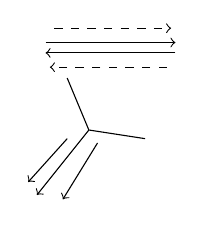
\begin{tikzpicture}[scale=.55]
\draw[->] (0,.12)--(3,.12);\draw[->] (3,-.12)--(0,-.12);\draw[dashed,->] (.2,.45)--(2.9,.45);\draw[dashed,->] (2.8,-.45)--(.1,-.45);
\draw (1,-1.9)--(.5,-.7) (1,-1.9)--(2.3,-2.1);\draw[->] (1,-1.9)--(-.2,-3.4);\draw[->] (.5,-2.1)--(-.4,-3.1);\draw[->] (1.2,-2.2)--(.4,-3.5);
\end{tikzpicture}}
\margin{$\unsure{A}$}
\[
\boxed{\begin{aligned}
\sigma_1^C(\mathrm r\deleted{\unsure{\mathrm g}}\mathrm d(\vec a))&=\deleted{\unsure{\mathrm{rd}}}\mathrm{rg}(\rho_\Gamma^{-1}(\vec a))=\sigma_0^C\mathrm{rd}(\rho_\Gamma(\vec a))\\
\sigma_1(\mathrm r\deleted{\unsure{\mathrm d}}\mathrm g(\vec a))&=\mathrm r\deleted{\unsure{\mathrm g}}\mathrm d(\rho_\Gamma^{\deleted{\unsure{-1}}}(\vec a))\deleted{\unsure{=\sigma_0^C}}
\end{aligned}}
\]
\[
\deleted{\rho_{\unsure{s}}(\vec a)=}
\left\{\begin{aligned}
\rho_C(\mathrm{rd}\vec a)&=\mathrm{rd}(\rho_\Gamma^{\deleted{\unsure{-1}}}(\vec a))\\
\rho_C(\mathrm{rg}\vec a)&=\unsure{\mathrm g|\mathrm{rg}}(\rho_\Gamma^{-1}\deleted{\unsure{\sigma_\Gamma}}\vec a))
\end{aligned}\right.
\]
\margin{\uline{NB} La définition des \uline{contours} \uline{orientés} $C$ ne dépend que de $\vec A$ muni de $\unsure{\rho_C|\rho_\Gamma}$ (à l'exclusion de $\sigma_0$)}
\figure{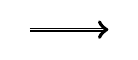
\begin{tikzpicture}\draw[double,->] (0,0)--(1,0);\end{tikzpicture}}

\unsure{Le} contour $C$ : \unsure{incidé} \unsure{sens} des \unsure{Aristyp.}

a) $C$ est orienté (``sens direct autour de $\Gamma$'')
\deleted{\deleted{\unsure{C}} $C'$ \unsure{par} ``\unsure{juxtaposition}'' i.e. \unsure{chaque} \inserted{(tient compte de $\unsure{o}$)} \unsure{est} \unsure{orientée}, soit la donnée d'une application \unsure{canonique}
\[
\vec A(C)'_+\subset\vec A(C),
\]
(``\unsure{plages} \unsure{topologiques}'') : \unsure{la} \unsure{unique} \unsure{p.}
\[
A(C)\longrightarrow\pm1
\]
\unsure{donnant} la valeur \unsure{$+1$ et $-1$} sur les deux \unsure{côtés}.}

\margin{i.e. on a\par
$\vec A=\vec A(C)_+\subset\vec A(C)$\par
ou\par
$\sigma_0\vec A=\vec A(C)_-$\par
$\sigma_1\vec A=\vec A(C)_-$}
Donc
\[
\left\{\begin{aligned}
\vec A(C)&\simeq\uline{\vec A(C)_+}\times\{\pm1\}\\
\sigma_0^C&\simeq\mathrm{id}\times\tau
\end{aligned}\right.
\]
La donnée de $\sigma_1^C$ revient à celle d'une permutation
\[
\rho_C=\{\vec a\longrightarrow\sigma_1^C(\sigma_0^C(\vec a))\}\quad\text{sur }\vec A.
\]
b) On a une involution, sans pts fixes $\sigma_\Gamma$ sur l'ens \deleted{\unsure{des}} des côtés de $C$, qui s'identifie à :
\[
\vec A=\vec A(C)_+.
\]
\mspage{7}

\scanpage{9}
{\ttfamily\scriptsize
\begin{tabular}{l}
J E S 2\quad J O B\quad L O G\quad --\quad S Y S T E M\quad E 3 3 3\quad --\quad N O D E\quad E 3 3 3\\[1ex]
16.39.12 J1125CNU\quad\$ J1125*PREDONTA STARTED - INIT 10 - CLASS Q - SYS E333\\
16.39.14 J1125CNU\quad DSN CISI.PROD.CSSBATCH.V1.YY01\\
16.39.14 J1125CNU\quad CSS2090 - JOB INPUT FILE TEMPORARILY FULL - PLEASE TRYAGAIN LATER\\
16.39.14 J1125CNU\quad SMF RECORD 153-1 (CLOSE) WRITTEN\\
16.39.15 J1125CNU\quad\$ J1125*PREDONTA ENDED\\[1ex]
------ JES2 JOB STATISTICS ------\\[1ex]
\quad 19 MAY 82 JOB EXECUTION DATE\\[1ex]
\hspace{1cm}26 CARDS READ\\[1ex]
\hspace{1cm}93 SYSOUT PRINT RECORDS\\[1ex]
\hspace{1cm}0 SYSOUT PUNCH RECORDS\\[1ex]
\hspace{.5cm}0.05 MINUTES EXECUTION TIME
\end{tabular}}
\mspage{\unsure{8|2}}

\scanpage{10}
\mspage{2'}
Ces deux données \deleted{\unsure{par}} sur le contour $C$ permettent de récupérer un graphe circularisé $\Gamma$, ayant $\vec A$ comme ens des arêtes orientées, avec opérations $\sigma_A$, $\rho_S$ données ainsi :
\[
\left\{\begin{aligned}
\sigma_\Gamma&=\sigma_C\\
\rho_\Gamma&=\rho_C
\end{aligned}\right.
\]

\uline{En résumé} La catégorie des graphes combinatoires circularisés $\Gamma$ (sans sommet isolé) \inserted{$(\vec A\deleted{\unsure{_\Gamma}}(\Gamma),\rho_\Gamma,\sigma_\Gamma)$} est équivalente à celle des contours orientés, avec involution \inserted{sans pt fixe $\sigma_C$} sur l'ens des \uline{arêtes}, soit $C$ ($=A(C)$ ens des arêtes de $C$, $\rho_C$ rotation fondamentale de $C$, $\sigma_C$ involution sur $A(C)$). \deleted{\unsure{par la}} \deleted{\unsure{p}} correspondance fondamentale :
\diagram{\begin{tikzcd}[row sep=large,column sep=large]
\vec A(\Gamma)&A(C)\arrow[l,"\sim"']\\
\sigma_\Gamma\arrow[r,leftrightarrow]&\unsure{\rho_C|\sigma_C}\\
\rho_\Gamma^{\unsure{\sigma|-1}}\sigma_\Gamma&\rho_C\arrow[l,maps to]\\
\rho_\Gamma&\rho_C\sigma_C\arrow[l,maps to]
\end{tikzcd}}
\margin{On appellera cela \uline{déploiement} \unsure{du} graphe plan donné}
\margin{$\rho_\Gamma^{\unsure{\sigma}}$ rotation renversée pour \unsure{la circ\({}^{\mathrm{on}}\) actuelle définie|le contour actuel défini} par $\Gamma$}

\begin{center}\fbox{\begin{minipage}{.92\linewidth}
$\Gamma$ un arbre $\Longleftrightarrow$ $C$ est un polygone comb. (non ponctuel), et l'involution $\sigma_C$ de $A(C)$ est totalement non pénétrante, i.e. pour deux \deleted{\unsure{paires}} \inserted{orbites} disjointes d'arêtes sous $\sigma_C$, \unsure{leur position|la partition} est n.p.
\end{minipage}}\end{center}
\mspage{\unsure{9|09}}

\scanpage{11}
\mspage{3}
\diagram{\begin{tikzcd}[row sep=huge]
{\begin{gathered}\text{``Arbres plans'' \inserted{(non ponctuels)}}\\\text{(dans un plan pas néc. \deleted{orienté})}\end{gathered}}\arrow[d,leftrightarrow,"\simeq"]\\
{\begin{gathered}\text{polygones combinatoires, avec \deleted{involution} inv. sans}\\\text{pts fixes non \unsure{pénétrante} sur l'ens des}\\\text{\deleted{sommets}\inserted{arêtes.}}\end{gathered}}
\end{tikzcd}}
\par\noindent\rule{\linewidth}{.4pt}

Revenant au cas d'un graphe $\Gamma$ circularisé \inserted{général}, Topologiquement, le graphe top. $|\Gamma|$ se déduit de $|C|$ par \deleted{les identifications} un quotient par la relation d'équivalence suivante : on recolle l'arête $a$ et l'arête $\sigma_Ca$, en \uline{renversant} les \unsure{orientations} induites sur ces arêtes.

Dans le cas où $\Gamma$ est un arbre, on peut interpréter celui-ci \inserted{top${}^{t}$} en considérant $C$ comme le bord d'un disque orienté $D$, \unsure{subdivisé} en arêtes, et en joignant les ``centres'' des arêtes qui se correspondent par $\sigma_C$, de façon à ce que les segments obtenus ne se rencontrent pas.
\figure{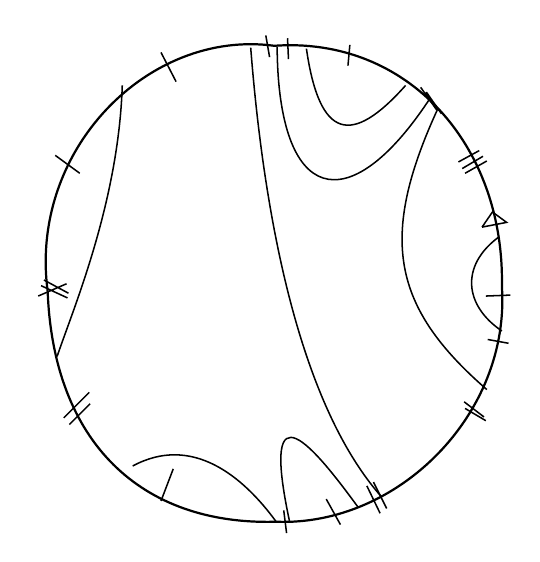
\begin{tikzpicture}[x=.012cm,y=-.012cm,line width=.55pt]
\draw[line width=.8pt] (95,1640).. controls (75,1490) and (202,1362)..(335,1380).. controls (476,1370) and (579,1485)..(576,1635).. controls (585,1770) and (466,1889)..(337,1884).. controls (194,1888) and (101,1800)..(95,1640);
\draw (174,1422).. controls (170,1547) and (121,1661)..(105,1709);
\draw (310,1382).. controls (326,1586) and (368,1766)..(448,1857);
\draw (338,1381).. controls (339,1547) and (413,1567)..(499,1437);
\draw (369,1383).. controls (383,1480) and (417,1486)..(474,1422);
\draw (508,1447).. controls (445,1584) and (460,1657)..(560,1744);
\draw (572,1583).. controls (532,1613) and (536,1655)..(576,1682);
\draw (185,1825).. controls (248,1791) and (302,1836)..(337,1884);
\draw (351,1883).. controls (319,1733) and (378,1806)..(424,1869);
\draw (215,1387)--(231,1418) (326,1369)--(330,1392) (349,1372)--(350,1394) (415,1379)--(413,1401);
\draw (490,1424)--(507,1448) (496,1429)--(512,1452);
\draw (530,1503)--(552,1491) (534,1510)--(556,1497) (537,1515)--(560,1502);
\draw (555,1572)--(581,1567)--(566,1556)--(555,1572);
\draw (559,1645)--(585,1644) (561,1691)--(583,1695);
\draw (536,1757)--(557,1773) (537,1764)--(559,1777);
\draw (433,1846)--(447,1875) (440,1842)--(454,1870);
\draw (390,1860)--(405,1887) (345,1872)--(348,1896) (228,1828)--(215,1862);
\draw (112,1774)--(139,1747) (118,1781)--(140,1759);
\draw (85,1645)--(115,1632) (88,1634)--(116,1647) (91,1628)--(117,1642);
\draw (103,1496)--(129,1515);
\end{tikzpicture}}
Les sommets de $\Gamma$ correspondent alors aux régions découpées dans $D$, et les arêtes orientées de $\Gamma$ aux frontières communes orientées,
\mspage{10}

\scanpage{12}
{\footnotesize\begin{tabular}{rlll}
\texttt{1}&\texttt{//PREDONTA}&\texttt{JOB '*********,00000000C','\hspace{4em}',}&\texttt{JOB 1125}\\
&\texttt{//}&\texttt{MSGLEVEL=(1,1)}&\\
\texttt{2}&\texttt{//}&\texttt{EXEC CSSBATCH}&\\
\texttt{3}&\texttt{XXCSSBATCH}&\texttt{PROC REG=100K,P=''}&\texttt{00010000}\\
\texttt{4}&\texttt{XXCSSBATCH}&\texttt{EXEC PGM=CRBATCH,REGION=\&REG,PARM=\&P}&\texttt{00020000}\\
\texttt{5}&\texttt{XXSTEPLIB}&\texttt{DD DSN=CISI.PROD.CSSBATCH.V1.YY01,DISP=SHR}&\texttt{00030003}\\
\texttt{6}&\texttt{XXSYSUT1}&\texttt{DD DSN=\&\&SYSUT1,UNIT=\unsure{SYSTSO|SYSTS0},SPACE=(TRK,30),DISP=(NEW,DELETE)}&\texttt{00031006}\\
\texttt{7}&\texttt{XXSYSUDUMP}&\texttt{DD SYSOUT=*}&\texttt{00040000}\\
\texttt{8}&\texttt{XXCRJIF}&\texttt{DD DSN=SYS1.CR.JIF,DISP=SHR}&\texttt{00050000}\\
\texttt{9}&\texttt{XXSYSIN}&\texttt{DD DDNAME=CRAYIN}&\texttt{00060000}\\
\texttt{10}&\texttt{//CRAYIN}&\texttt{DD *}&
\end{tabular}}
\mspage{11}

\scanpage{13}
\mspage{3'}
\unsure{donc|dont} le graphe $\Gamma$ exprime la façon dont les régions se rencontrent suivant des frontières communes.

La catégorie des arbres plans \inserted{(pas néc. plans orientés)} est équivalente \unsure{à|:} la catégorie isotopique des disques \deleted{orientés} (pas néc. orientés donc) munis d'un tel découpage. Le polygone combinatoire \deleted{\unsure{le contour}} \inserted{$C$} est \uline{dual} de celui défini par les cordes du découpage sur le bord des disques, les sommets de $\Gamma$ correspondant à des paquets d'arêtes de ce contour (celles qui bordent une région déterminée du découpage \deleted{\unsure{du}} du disque).
\mspage{12}

\cotefile{120}
\scanpage{1}
\begin{minipage}{0.55\linewidth}
{\Huge\bfseries IMAG}\par
INSTITUT MONTPELLIERAIN\par
ALEXANDER GROTHENDIECK
\end{minipage}\hfill
\begin{minipage}{0.43\linewidth}
\figure{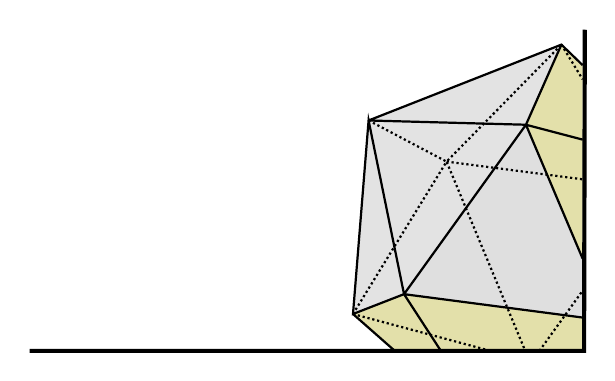
\begin{tikzpicture}[x=0.009cm,y=-0.009cm]
\fill[gray!22] (28,110)--(300,3)--(250,116)--(78,355)--(6,383)--cycle;
\fill[gray!25] (78,355)--(250,116)--(330,137)--(330,310)--(330,435)--(130,435)--cycle;
\fill[olive!25] (300,3)--(330,32)--(330,305)--(250,116)--cycle;
\fill[olive!25] (6,383)--(78,355)--(330,388)--(330,435)--(65,435)--cycle;
\draw[thick] (28,110)--(300,3)--(330,32) (28,110)--(250,116)--(300,3) (250,116)--(330,137) (250,116)--(330,305) (250,116)--(78,355)--(6,383)--(28,110)--(78,355)--(130,435) (78,355)--(330,388) (6,383)--(65,435);
\draw[densely dotted,thick] (28,110)--(138,168)--(300,3) (138,168)--(330,193) (6,383)--(138,168)--(249,435) (6,383)--(200,435) (269,435)--(330,350) (300,3)--(330,52);
\draw[line width=1.5pt] (-450,435)--(332,435)--(333,-18);
\end{tikzpicture}}
\end{minipage}

\scanpage{2}
\margin{\unsure{1/18|118}}
\uline{\deleted{\unsure{Structures}}\inserted{Topologie} modérée}

(Autour de l'Eloge)
\mspage{1}

\scanpage{3}
\mspage{1}
\margin{\textcircled{I}\par\uline{Modèles modérés} \deleted{\unsure{et espaces}}\inserted{ens} \deleted{modérés}}
\[
\forall n\in\mathbb N^*,\qquad\mathcal M_n\subset\mathcal P(R^n)
\]
\textcircled{\scriptsize$M1$} $\forall u:[1,n]\longrightarrow[1,m]$, d'où $u^*:R^m\longrightarrow R^n$, on a
\[
u^*(\mathcal M_m)\subset\mathcal M_n\qquad\text{i.e.}\quad\forall A\in\mathcal M_m,\text{ on a }u^*(A)\in\mathcal M_n.
\]
\textcircled{\scriptsize$M2$} $\forall u:[1,n]\longrightarrow[1,m]$ \uline{surjectif}, d'où $u^*:R^m\hookrightarrow R^n$ injectif, on a
\[
u^{*-1}(\mathcal M_n)\subset\mathcal M_m\qquad\text{i.e.}\quad\forall \unsure{B|A}\in\mathcal M_n,\text{ on a }u^{*-1}(\unsure{B|A})\in\mathcal M_m.
\]
\margin{donc si on a $M1$, \unsure{on trouve}\par $A\in\mathcal M_m\Longleftrightarrow\unsure{u_*|u^*}(A)\in\mathcal M_n$}
\textcircled{\scriptsize$M3$} $\forall u:[1,n]\longrightarrow[1,m]$ d'où $u^*:R^m\longrightarrow R^n$, et pour $A\in\mathcal M_m$, $B\in\mathcal M_n$, on a
\[
u^{*-1}(B)\cap A\in\mathcal M_m
\]
\textcircled{\scriptsize$M4$} $\forall A\in\mathcal M_m$, $B\in\mathcal M_n$, on a (modulo $R^m\times R^n\simeq R^{m+n}$)
\[
A\times B\in\mathcal M_{m+n}.
\]

\uline{Commentaires} \textcircled{1} $M1)$ permet de définir, pour \deleted{tout} $I$ ens fini non vide, $\mathcal M_I\in\mathcal P(R^I)$, et alors on a des propriétés $M'1$ à $M'4$ pour les $\mathcal M_I$ et les $u:I\unsure{-|\longrightarrow}J$.

\textcircled{2} : Pour avoir $M1$, il suffit de le supposer pour les \deleted{trois} cas :

a) $m=n$, $u\in\unsure{\mathfrak S_n}$

b) $m=n+1$, $u$ injectif (``op. face''), donc $u^*$ surjectif

c) $n=m+1$, $u$ surjectif \deleted{\unsure{(``op. dégénérescence'')}} \inserted{(``op dégénérescence'')} donc $u^*$ injectif

\deleted{\unsure{et en} seulement les \unsure{projections} \unsure{dans}}

\margin{ou $\overline{\mathrm m}$ seulement les op. standard\par
$R^n\longrightarrow R^{n+1},\ (x_1,\ldots,x_n)\longmapsto(x_1,\ldots,x_n,x_n)$\par
et\par
$R^{n+1}\unsure{\longrightarrow|-}R^n,\ (x_1,\ldots,x_{n+1})\longmapsto(x_1,\ldots,x_n)$}

Pour avoir $M2$, il suffit de le supposer pour les op${}^{\unsure{\mathrm{os}|\mathrm{o}}}$ de dégénérescences, \inserted{et \unsure{$\overline{\mathrm m}$|m} seulement pour l'application \deleted{\unsure{$R^n\hookrightarrow R^{n+1}$}} \figure{
\begin{tikzpicture}[x=.12cm,y=.12cm,baseline=-.5ex]\draw[line width=1.2pt] (0,0)--(.7,3) (.45,1.1)--(1.6,.2)--(.3,.6)--(1.1,1.6);\end{tikzpicture}}}
\margin{\figure{
\begin{tikzpicture}[x=.12cm,y=.12cm]\draw[line width=1.2pt] (0,0)--(.7,3) (.45,1.1)--(1.6,.2)--(.3,.6)--(1.1,1.6);\end{tikzpicture}}\par
\fbox{$\begin{gathered}R^n\hookrightarrow R^{n+1}\\(x_1,\ldots,x_n)\deleted{\unsure{x_n}}\\\longmapsto(x_1,\ldots,x_n,x_n)\end{gathered}$}}
Notons que $M1$, $M2$, $M4$ impliquent que les $\unsure{\mathfrak S_n|\mathcal M_n}$ sont stables par intersection de deux
\[
A,B\in\unsure{\mathfrak S_n|\mathcal M_n}\Longrightarrow A\cap B\in\unsure{\mathfrak S_n|\mathcal M_n}
\]
\inserted{(uniquement $M1$, $M2$, $M4$)}
d'où résulte que pour avoir $M3$, il suffit de le prouver pour $u$ \unsure{surjectif|injectif}, et $\overline{\mathrm m}$ seulement pour $u^*$ l'op. standard
\[
R^{n+1}\unsure{-|\longrightarrow}R^n,\quad(x_1,\ldots,x_{n+1})\longmapsto(x_1,\ldots,x_n).
\]
\mspage{2}

\scanpage{4}
En résumé on voit que $M1$, $M2$, $M3$ peuvent être remplacés par

a) \deleted{$\unsure{\forall n}\ \forall\sigma\in\mathfrak S_n$} $\forall n\in\mathbb N^{\unsure{0|*}}$, $\sigma\in\mathfrak S_n$, $A\in\mathcal M_n$, on a $\sigma^*(A)\in\mathcal M_n$

b) $\forall n\in\mathbb N^*$, d'où
\[
\alpha_n:[1,\ldots n+1]\longrightarrow[1,n]\qquad
\left\{\begin{gathered}\text{identité sur }[1,n]\\ n+1\longmapsto n\end{gathered}\right.
\]
d'où \deleted{$\unsure{R}$}
\[
\alpha_n^*:R^n\hookrightarrow R^{n+1}\qquad(x_1,\ldots,x_n)\longmapsto(x_1,\ldots,x_n,x_n),
\]
on a
\[
\begin{aligned}
b_1)\quad&\forall A\in\mathcal M_n,\quad\alpha_n^*(A)\in\mathcal M_{n+1},\\
b_2)\quad&\forall B\in\mathcal M_{n+1},\quad\alpha_n^{*-1}(B)\in\mathcal M_n
\end{aligned}
\]
c) $\forall n\in\mathbb N^*$, d'où $\beta_n:[1,n]\hookrightarrow[1,n+1]$ inclusion can., d'où
\[
\beta_n^*:R^{n+1}\longrightarrow R^n,\quad(x_1,\ldots,x_{n+1})\longmapsto(x_1,\ldots,x_n),
\]
on a
\[
\begin{aligned}
c_1)\quad&\forall A\in\mathcal M_{n+1},\ B\in\mathcal M_n,\text{ on a }A\cap\beta_n^{*-1}(B)\in\mathcal M_{n+1}\\
c_2)\quad&\forall A\in\mathcal M_{n+1},\quad\beta_n^*(A)\in\mathcal M_n
\end{aligned}
\]

\textcircled{3} $M1$ implique que si un des $\mathcal M_n$ est vide, tous le sont -- et alors les axiomes $M1$ à $M4$ sont satisfaits trivialement. On va exclure ce cas \inserted{trivial}, i.e. supposer
\[
(*)\qquad\mathcal M_1\ne\varnothing.
\]
$\unsure{M1|M4}$ implique que si un des $\mathcal M_n$ contient $\varnothing$, tous le contiennent. Si ce n'est pas le cas, alors chaque $\mathcal M_n$ (étant stable par intersection de deux ens) est une base de filtre sur $R^n$.

On exclut ce cas, i.e. on suppose la relation suivante, plus forte que $(*)$
\[
(**)\qquad\varnothing\in\mathcal M_1\qquad(\text{d'où }\varnothing\in\mathcal M_n\quad\forall n\in\mathbb N)
\]
\uline{NB} Si cette propriété \unsure{n'étant|n'était} vérifiée, les présents
\mspage{3}

\scanpage{5}
\mspage{2}
\[
\mathcal M'_n=\mathcal M_n\cup\{\varnothing\}
\]
les $\mathcal M'_n$ satisfont encore les axiomes \ldots

\deleted{\textcircled{4} \unsure{On a} \unsure{NB} \unsure{Si on pose}}

De $\overline{\mathrm m}$, \deleted{$\unsure{M}$} $M1$ implique que si on a, pour \uline{un} $n$, \deleted{$\unsure{M}$} $\mathcal M_n=\{\varnothing\}$, alors c'est vrai aussi pour $\forall n$ -- cas trivial \inserted{(qui satisfait aux axiomes)} que je vais exclure. Donc je suppose aussi
\[
(***)\quad\deleted{\unsure{\exists}}\ \mathcal M_1\ne\{\varnothing\}\quad\text{i.e.}\quad\exists A\in\mathcal M_1,\quad A\ne\varnothing.
\]
Ceci étant, si on pose pour $I\unsure{\ne|=}\varnothing$
\[
\mathcal M_\varnothing=\mathcal P(\underbrace{R^\varnothing}_{\text{espace ponctuel }\{e\}})=\{\varnothing,\{e\}\}
\]
\margin{les propriétés $M'1$ à $M'4$ (cf \textcircled{1}) restent satisfaites sans se borner à \deleted{\unsure{$I,J$}} $I,J\ne\varnothing$}

\textcircled{4} Soit \deleted{$\unsure{x\in R_n}$}
\[
x=(x_1,\ldots,x_n)\in R^n
\]
alors il résulte de $M1$ et $M4$ que
\[
\{x\}\in R^n\Longleftrightarrow\forall i\in[1,n],\text{ on a }\{x_i\}\in\mathcal M_1.
\]
Soit
\[
R_0=\{x\in R\mid\{x\}\in\mathcal M_1\}\qquad\text{donc }R_0\subset R,
\]
alors pour $\forall$ ens fini $I$, on a
\[
R_0^I=\{x\in R^I\mid\{x\}\in\mathcal M_I\}
\]
\inserted{$\widehat R^I$}
Notons que si \deleted{$R_0\ne\varnothing$} \inserted{$\mathrm{Card}\ R_0\ge2$}, alors on conclut de la stabilité \inserted{de $\mathcal M_1$} par intersection que $\varnothing\in\mathcal M_1$, donc on satisfait à \textcircled{3}.

\textcircled{5} Exemples (à part $\mathcal M_n=\varnothing\quad\forall n$, et $\mathcal M_n=\{\varnothing\}\quad\forall n$)
\mspage{4}

\scanpage{6}
a) $\mathcal M_n=$ parties de cardinal $\le1$ de $R^n$

b) $\mathcal M_n=$ parties finies de $R^n$

c) $\mathcal M_n=$ toutes les parties de $R^n$

\margin{ici les axiomes a), b), c) du NB \textcircled{2}, \uline{à l'exclusion} de $c_2)$}

Aucun de ces exemples n'est particulièrement \unsure{passionnant}.

\margin{\textcircled{II} \uline{espaces modérés}\par
Dans ce qui suit \unsure{au lieu de} $(M1)$ il suffit l'axiome concernant \deleted{\unsure{injections|les applications}} \inserted{\unsure{les surjections}} \uline{pour les seuls} $[1,n]$ -- \unsure{c.-à-d. les} \unsure{linéaires des s.} \illegible{3} \unsure{applications} \unsure{des} \uuline{\unsure{directes}}.}
\margin{on n'exclut \unsure{pas} $I$ vide}

Terminologie : partie modérée de $R^I$, points modérés de $R$, de $R^I$.

\uline{déf} Soit $A\in\mathcal M_I$, $B\in\mathcal M_J$, $f:A\unsure{\longrightarrow|-}B$, d'où
\[
\Gamma_f\subset A\times B\subset R^I\times R^J\simeq R^{I\unsure{\cup|\amalg}J}.
\]
On dit que $f$ est \uline{modérée} si
\[
\Gamma_f\in\mathcal M_{I\unsure{\cup|\amalg}J}.
\]

\margin{\unsure{via|vu} $M2$}
\uline{Proposition} a) $\mathrm{id}_A$ (si $A\in\mathcal M_I$) est modérée

b) \diagram{\begin{tikzcd}[row sep=tiny,column sep=large]
f:A\arrow[r,no head]&B&\text{et}&g:B\arrow[r,no head]&C\\
\mathcal M_I\arrow[u,phantom,"\rotatebox{90}{\(\in\)}" description]&\mathcal M_J\arrow[u,phantom,"\rotatebox{90}{\(\in\)}" description]&&&\mathcal M_{\unsure{K|n}}\arrow[u,phantom,"\rotatebox{90}{\(\in\)}" description]
\end{tikzcd}} modérés $\Longrightarrow gf$ modéré

c) \diagram{\begin{tikzcd}[row sep=tiny]
f:A\arrow[r]&B\\
\mathcal M_I\arrow[u,phantom,"\rotatebox{90}{\(\in\)}" description]&\mathcal M_J\arrow[u,phantom,"\rotatebox{90}{\(\in\)}" description]
\end{tikzcd}} modéré et bijectif $\Longrightarrow f^{-1}$ modéré

D'où catégorie des \uline{modèles modérés} $\mathrm{Mod}_{\mathcal M_*}$, \inserted{(on prend $(I,A\in\mathcal M_I)$)} et un foncteur \uline{conservatif} \uline{fidèle}
\diagram{\begin{tikzcd}
\mathrm{Mod}_{\mathcal M_*}\arrow[r]&(\mathrm{Ens})
\end{tikzcd}}\qquad$(I,A)\longmapsto A$.
\margin{on n'exclut pas les modèles $\subset R^0=\{e\}$, \inserted{modèle} \deleted{\unsure{espace|discret}} réduit à un point \ldots}

On en déduit\deleted{\unsure{on}} la catégorie des ensembles \inserted{(ou ``espaces'')} $(\mathcal M_*-)$ modérés, équivalente à : $\mathrm{Mod}_{\mathcal M_*}$, mais avec un foncteur
\diagram{\begin{tikzcd}
\deleted{\unsure{\mathrm{Mod}}}\ \mathrm{Esp}_{\mathcal M_*}\arrow[r]&(\mathrm{Ens})
\end{tikzcd}}\qquad$X\longmapsto|X|$
qui est fidèle, conservatif et de plus ``transportable'', i.e.
\mspage{5}

\scanpage{7}
\mspage{6}\hfill\mspage{3}
pour tout diagramme
\diagram{\[
\left\{\begin{gathered}\begin{tikzcd}[row sep=large]
X&\\
{|X|}\arrow[r,"{\substack{\alpha\\\sim}}"]&E
\end{tikzcd}\end{gathered}\right.
\]}
avec $X\in\mathrm{Ob}\,\mathrm{Esp}_{\mathcal M_*}$, $\exists$ une unique \deleted{$Y$ et} flèche $f:X\unsure{-|\longrightarrow}Y$ de $\mathrm{Esp}_{\mathcal M_*}$, qui relève $\alpha$ (``Transport de structure'').

\uline{Proposition} Dans la catégorie $\mathrm{Esp}_{\mathcal M_*}$ des espaces $\mathcal M_*$-modérés, il y a des
\deleted{produits \unsure{fibrés|finis}, et des produits (de deux objets), et le foncteur $X\longmapsto|X|$ y commute. Si on suppose
\[
(\unsure{M5'|M5})\qquad R_0\ne\varnothing
\]
alors il \deleted{foncteur} y a aussi un objet final (qui est uniponctuel) et \unsure{le} \unsure{foncteur}}
\inserted{(\deleted{\unsure{pas des objets}} \unsure{sans restriction})}
\inserted{\unsure{des limites finies}}
et le foncteur $X\longmapsto|X|$ commute.
\margin{\unsure{trivialité de} \unsure{celui} \illegible{1} d'un \illegible{1} \unsure{des} \unsure{lois} \illegible{2} des \unsure{foncteurs}}

\uline{Proposition} Si pour \uline{un} $n\in\mathbb N^*$ on a \deleted{$\unsure{R}$} $R^n\in\mathcal M_n$, alors \unsure{c'est} vrai pour $\forall n$, \unsure{et même} pour $\forall I$ fini
\[
R^I\in\mathcal M_I.
\]
Considérons l'axiome (\uline{facultatif})
\[
\deleted{\unsure{M5}}(M0)\qquad R\in\mathcal M_1\qquad(\Longrightarrow\forall I\in(\mathrm{Ens\ fini}),\ R^I\in\mathcal M_I)
\]
\margin{Quand on n'a pas $(M0)$, mais que l'on suppose $(M5)$, alors la \unsure{réunion} des $A\in\mathcal M_1$, \unsure{fait que} $\unsure{R'}$ est \unsure{obtenu} \unsure{comme} \illegible{2} \unsure{de} $\unsure{R}$ \unsure{réunion} \unsure{filtrante} \illegible{2}.\par
\unsure{On dispose} de \unsure{ces} \unsure{ens.} \unsure{stables} \illegible{2} \unsure{l'axiome} $(M1)$ \unsure{réciproque} \illegible{1} \unsure{l'influence} \unsure{de} \unsure{foncteurs} \illegible{2}.\par
\unsure{comme} $(M5)$ \unsure{l'expression} \unsure{espace} \unsure{muni de} \unsure{l'} $\unsure{R}$ \unsure{aussi} \unsure{vide} \unsure{annulé}.}
\margin{\unsure{objet} \unsure{abs.} \unsure{Cat}\uline{\unsure{f}}}

\scanpage{8}
Alors $R$ est muni d'une structure modérée canonique (en tant que modèle $\subset R^1=R$), i.e.
\[
 R\in\operatorname{Ob}\mathcal E\qquad(\mathcal E=\operatorname{Esp}_{\mathcal M_*})
\]
et $\forall$ objet de $\mathcal E$ est isomorphe à un sous-objet d'un $R^n$ \inserted{(produit dans $\mathcal E$)}. On récupère $\mathcal M_n$ comme l'ens des sous-objets \inserted{\unsure{sous-ens.} de $R^n$ \unsure{correspondants dans Ens}} (dans $\mathcal E$) de l'objet $R^n$. On trouve que la donnée d'un $\mathcal M_*$ est équivalente à la donnée d'un système (à isom. près)
\[
 (\mathcal E,R,X\longmapsto |X|)
\]
de a) la catégorie $\mathcal E$ avec $\varprojlim$ finies

b) le foncteur $X\mapsto |X|$ $\mathcal E\longrightarrow(\mathrm{Ens})$ exact à gauche

c) l'objet $R\in\operatorname{Ob}\mathcal E$ tel que $\forall$ objet de $\unsure{R|\mathcal E}$ se plonge dans un $R^n$.

\margin{Parler aussi des applications modérées d'ens. modérés dans des $R^I$.}

\margin{Introduire les parties modérées d'un espace modéré \unsure{correspondant} aux sous-objets dans $\operatorname{Esp}_{\mathcal M_*}$, les propriétés de stabilité $f(A)$, $f^{-1}(B)$, produits cartésiens.}

\figure{\begin{tikzpicture}\node[draw,ellipse] {III};\end{tikzpicture}}
\uline{Limites inductives finies d'\unsure{espaces} modérés}

S'intéresser à la question des réunions finies des parties modérées, et des $\varinjlim$ finies dans $(\operatorname{Esp}_{\mathcal M_*})$.

\margin{A partir d'ici, \unsure{on suppose que|je n'utilise} $\unsure{M4|M5}$ \unsure{de} \unsure{réunion} \unsure{seulement} \unsure{possible}. \unsure{Je verrai} $(M)_0$ pour \unsure{la suite|les suites} \unsure{par un axiome}.}
\mspage{7}

\scanpage{9}
\mspage{4}
\margin{\unsure{le donner} \uline{après} la proposition qui suit, \unsure{ou postuler}\ldots}
\uline{Proposition} Si \deleted{$R_0\ne\varnothing$}, \inserted{$\operatorname{Card}R_0\geq2$}, \deleted{\unsure{alors} \unsure{(si $R\in\mathcal M_1$)}, \unsure{$\mathcal E$} \unsure{dans}} $\mathcal E$
\deleted{\unsure{existe un} \unsure{$(\operatorname{Hom}_{\mathcal E}(e,R))$} \unsure{de l'objet} \unsure{$R_0$}}
\deleted{$\operatorname{Hom}_{\mathcal E}(\underset{\inserted{\substack{\unsure{\shortparallel|''}\\\{e\}}}}{R^0},R)\ne\varnothing$} dans \unsure{des}
\deleted{$\mathcal E$ \unsure{est}, \unsure{a des} sommes finies} \unsure{(uniquement} et $X\mapsto|X|$ y commute.

\figure{\begin{tikzpicture}\node[draw,ellipse] {$M5$};\end{tikzpicture}}
\uline{Corollaire} Sur $\forall$ ens fini il $\exists$ une structure modérée et une seule, pour laquelle les parties uniponctuelles soient modérées (str. mod. discrète).

\unsure{On se propose} le cas où on veut construire $X_1\amalg_Z X_2$, sans supposer $Z$ vide. Notons d'abord ceci :

\uline{Proposition} Soit $I$ un \deleted{type de} \inserted{type de} diagrammes fini, et $(X_i)_{i\in I}$ un diagramme de type $I$ dans $\mathcal E=\operatorname{Esp}_{\mathcal M_*}$, i.e. d'espaces modérés. Soit $X$ la limite inductive \uline{dans} $(\mathrm{Ens})$, qui est donc un \inserted{certain} quotient de $\coprod X_i$ (comme toujours). Supposons qu'il existe sur $X$ une structure modérée, telle que les appl. can. $g_i:X_i\longrightarrow X$ soient modérées. Alors $X$, muni de cette structure, est \inserted{une} $\varinjlim_I$ des $X_i$.
\mspage{8}

\scanpage{10}
Axiome supplémentaire
\[
 (M5)\quad \forall n,\quad \mathcal M_n\text{ stable par réunions finies}
\]
\[
 (\Longleftrightarrow\ \varnothing\in\mathcal M_n,\ \deleted{\unsure{\delta}}\text{ et }A,B\in\mathcal M_n\Longrightarrow A\cup B\in\mathcal M_n)
\]
\uline{Proposition} Parties modérées d'un esp. mod. stable par réunions finies.

\uline{Proposition} Sur $\varnothing$ il $\exists$ une structure modérée unique, qui en fait objet initial de $\operatorname{Esp}_{\mathcal M_*}$.

\uline{Proposition} Soit $X$ un espace modéré, $(X_i)_{i\in I}$ une famille finie de parties modérées de $X$. Alors $\bigcup X_i$ est une partie modérée de $X$. Si $X=\bigcup_iX_i$, alors $X$ est somme amalgamée des $X_i$ suivant les $X_i\cap X_j$ --- une application $f:X\longrightarrow Y$ \inserted{entre espaces modérés} est modérée ssi ses restrictions aux $X_i$ le sont.

\uline{Question} Donnons-nous
\diagram{\begin{tikzcd}[column sep=small]
&\unsure{Y|Z}\arrow[dl]\arrow[dr]&\\
X_1&&X_2
\end{tikzcd}}
dans $\operatorname{Esp}_{\mathcal M_*}$, existe-t-il une somme amalgamée ? Si $Y=\varnothing$, c'est la question de l'existence des sommes finies dans $(\operatorname{Esp}_{\mathcal M_*})$.
\mspage{9}

\scanpage{11}
\mspage{5}
Pour que la somme amalgamée existe dans \deleted{\unsure{$\operatorname{Esp}$}} $\mathcal E$ et que $X\mapsto|X|$ y commute, il \unsure{f. et s.} qu'il existe une famille finie de \inserted{paires de} fonctions
\[
\begin{array}{l}
f_\alpha:\deleted{\unsure{g}}\ X_1\unsure{-|\longrightarrow}R\\
g_\alpha:X_2\unsure{-|\longrightarrow}R
\end{array}
\]
telles que l'on ait
\[
\text{a)}\quad f_\alpha(\unsure{i_1|z_1}(z))=g_\alpha(i_2(z))\qquad\forall\alpha\in\unsure{I|A},\ z\in Z
\]
b) \deleted{Si $\unsure{x},y$ les $f_\alpha$ \unsure{x}} les $f_\alpha$ ($g_\alpha$) séparent \deleted{$(f_\alpha)$} les pts de $X_1$ ($X_2$) i.e.
\[
 X_1\longrightarrow R^I\qquad(X_2\longrightarrow R^I)
\]
sont injectifs
\[
\begin{array}{ll}
\text{c)}&\text{Si }x_1\deleted{\unsure{\alpha}}\in X_1\smallsetminus i_1(Z)\\
&x_2\in X_2\smallsetminus i_2(Z)\\
&\exists\alpha\text{ avec }f_\alpha(x_1)\ne g_\alpha(x_2)
\end{array}
\]

\uline{NB} On peut généraliser, sous les conditions de la proposition, il existe la structure modérée qu'on veut sur $X$, ssi $\exists$ une famille finie $(F_\alpha)$ \deleted{\unsure{de}} de systèmes inductifs
\[
 (f_\alpha:i\in I\qquad f_{\alpha i}:X_i\underset{\text{modérée}}{\longrightarrow}R),
\]
déterminant des
\[
 f_\alpha:X\longrightarrow R
\]
telles que les $f_\alpha$ séparent les pts de $X$, i.e.
\[
 f=(f_\alpha):X\hookrightarrow R^A
\]
\mspage{10}

\scanpage{12}
En effet, si $Y$ est un espace modéré, une \deleted{\unsure{biject.|flèche}} \unsure{flèche} du syst. inductif $(X_i)$ (dans $\mathcal E$) dans $Y$, \inserted{$(f_i:X_i\longrightarrow Y)_{i\in I}$}, équivaut à la donnée d'une application $f:X\longrightarrow Y$, telle que les $f\circ g_i$ soient modérées. Il nous reste à prouver que cela implique que $f$ est modérée, i.e. que son graphe $\Gamma_f\subset X\times Y$ est une partie modérée. Or $X$ étant la réunion des images des $X_i$, il en est que $\Gamma_f$ est la réunion des images des $\Gamma_{f_i}\subset X_i\times Y$ par
\[
 X_i\times Y\xrightarrow{g_i\times\operatorname{id}_Y}X\times Y.
\]
Mais ces images sont modérées, et \deleted{donc} leur réunion aussi.

\uline{Cor} Soit $f:X\longrightarrow Y$ application modérée, $\mathcal R_f$ la relation d'équivalence définie par $f$ (qui est donc une partie modérée de $X\times X$, et est une $\mathcal E$-relation d'équivalence). Alors $X/\mathcal R_f$ existe dans $\mathcal E=\operatorname{Esp}_{\mathcal M_*}$, et est \inserted{can} isomorphe à $f(X)$ (avec structure induite)

\deleted{\uline{Cor. 2} Considérons}
\deleted{\diagram{\begin{tikzcd}[column sep=small]
&\deleted{Z}\arrow[dl,"\deleted{i_1}"']\arrow[dr,"\deleted{i_2}"]&\\
\deleted{X_1}&&\deleted{X_2}
\end{tikzcd}}}
\deleted{dans $\mathcal E$.}
\mspage{11}

\scanpage{13}
\mspage{6}
On va introduire
\[
(M6)\quad \deleted{\unsure{\exists f}}\quad
\forall Z,X\in\mathcal M_n,\quad Z\subset X,\quad\exists(f_\alpha)_{\alpha\in A}
\]
famille finie de fonctions modérées $X\longrightarrow R$ et des $(e_\alpha)_{\alpha\in A}$, $e_\alpha\in R_0$, telle que
\[
 Z=\bigcap f_\alpha^{-1}(e_\alpha).
\]
De plus, \unsure{OPS} que les $f_\alpha$ séparent les points de $X\smallsetminus Z$.

\margin{\uline{Prop} $(M6)$, $(M7)$ impliquent l'existence de la somme amalg. \unsure{avec une} \unsure{flèche|rétraction} \unsure{libre}.}
\margin{\diagram{\begin{tikzcd}[column sep=small]
X_1&Z\arrow[l,hook']\arrow[r]&X_2
\end{tikzcd}}}

\deleted{Cela implique que l'on peut faire un diagramme \inserted{cart}}
\deleted{\diagram{\begin{tikzcd}
\deleted{X}\arrow[r,hook]&\deleted{R^n\times R^A}\\
\deleted{Z}\arrow[u,hook]\arrow[r,hook]&\deleted{R^n\times\{e\}}\arrow[u,hook]
\end{tikzcd}}}
\deleted{$e=(e_\alpha)_{\alpha\in A}$}

\deleted{Appliquons ceci : $Z_1\unsure{\hookrightarrow|\longleftrightarrow}X_1$ et $Z_2\hookrightarrow X_2$}

\unsure{ce qui est} \uline{équivalent} au fait que le quotient $X/Z$ (contraction de $Z$ en un point) existe dans $\mathcal E$ au sens strict (i.e. $X\mapsto|X|$ y commute). De plus, on suppose
\margin{\unsure{Voir important}}
\[
(M7)\quad\forall Z,X\in\mathcal M_n,\quad Z\subset X,\quad\text{et }\forall
\]
\[
f:Z\longrightarrow R\text{ modérée},\qquad\exists g:X\longrightarrow R\text{ modérée}
\]
qui prolonge

\uline{Proposition} Moyennant $M5,M6,M7$, les sommes amalgamées $X_1\amalg_Z X_2$ ($Z\hookrightarrow X_1$, $Z\hookrightarrow X_2$) existent dans $\operatorname{Esp}_{\mathcal M_*}$, et commutent au foncteur oubli.
\margin{cf généralisation qui \unsure{vient} ci-dessous.}
\mspage{12}

\scanpage{14}
Soit $Z\hookrightarrow R^{\deleted{\unsure{n}}\inserted{I}}$ un plongement modéré. On peut (par $M7$) le prolonger en
\[
 X_i\longrightarrow R^I\qquad(i\in\{1,2\})
\]
Soit
\[
 X_i\unsure{-|\longrightarrow}R^{A_i}\qquad i\in\{1,2\}
\]
comme dans $M6$ (d'où un \deleted{\unsure{appl.}} plongement modéré $X_i/Z_i\hookrightarrow R^{A_i}$, \inserted{$Z_i=\unsure{u_i|i_i}(Z)$}), on a donc un : $X_1\longrightarrow R^{I\amalg A_1}$ qui est un plongement et s'insère dans un diagramme cartésien
\par\noindent\diagram{\begin{tikzcd}
X_1\arrow[r,hook,no head]&R^{I\amalg A_1}=R^I\times R^{A_1}\\
Z\arrow[u,hook,no head]\arrow[r,hook,no head]&R^I\times\{e_1\}\arrow[u,hook]&e_1\in R_0^{A_1}
\end{tikzcd}}\par
et de $=$ pour $X_2$, \deleted{\unsure{on le}} qu'on peut considérer comme \deleted{\unsure{des}} s'insérant dans
\deleted{\par\noindent\diagram{\begin{tikzcd}[column sep=small]
\deleted{X_1}\arrow[r,hook]\arrow[d]&\deleted{R^I\times R^{A_1}\times\{e_2\}}\arrow[r]\arrow[d]&\deleted{R^I\times R^{A_1}\times R^{A_2}}\\
\deleted{Z}\arrow[r]&\deleted{R^I\times\{e_1\}\times\{e_2\}}&\deleted{R^I\times\unsure{R^{A_2}|R^{A_1}}\times R^{A_2}}\arrow[u]
\end{tikzcd}}\par}
\par\noindent(*)\quad\diagram{\begin{tikzcd}[column sep=small,row sep=small]
X_1\arrow[r,hook]&R^I\times R^{A_1}\times\{e_2\}\arrow[r,hook,no head]&R^I\times R^{A_1}\times R^{A_2}\\
& R^I\times\{e_1\}\times\{e_2\}\arrow[u,hook]\arrow[r,hook]&R^I\times\{e_1\}\times R^{A_2}\arrow[u,hook,no head]\\
Z\arrow[uu,hook]\arrow[rr,hook]&&X_2\arrow[u,hook,no head]
\end{tikzcd}}\par
\mspage{13}

\scanpage{15}
\mspage{14}\mspage{7}
\margin{on suppose $M5$ mais pas $M6$ \unsure{et} $M7$}
\figure{\begin{tikzpicture}\node[draw,ellipse] {IV};\end{tikzpicture}}
Ind-structures modérées strictes \inserted{\uline{indespaces modérés}} \inserted{(ou ind-espaces modérés)} : consiste : la donnée d'un ens. $E$, et un ens de parties $\mathcal M_E$ de $E$ (les parties modérées), stable par réunions finies, \inserted{de réunion $E$}, avec une structure modérée sur chacun, ces structures s'induisant mutuellement, et
\[
 A\in\mathcal M,\quad B\in\mathcal M_A\Longrightarrow B\in\mathcal M.
\]
Il revient au $=$ de se donner la notion d'application modérée d'un $X$ modéré dans $E$, avec \deleted{\unsure{une identité}} quelques conditions \unsure{supplém.}. Si on suppose
\[
 (M8)\quad R\text{ est réunion \inserted{(filtrante par $M5$)} de ses parties modérées},
\]
on trouve une structure ind-modérée canonique sur $R$, et de $=$ sur les $R^I$.

\uline{Proposition} La catégorie des \inserted{$\overset{\unsure{\sim|\leftrightarrow}}{\underrightarrow{\operatorname{Esp}}}_{\mathcal M_*}$} \deleted{Ind} Ind-espaces modérés stricts admet des $\varprojlim$ finies, le foncteur oubli y commute.
\margin{\unsure{des ensembles modérés}}
\margin{$M1:M5$}
\margin{$\underrightarrow{\operatorname{Esp}}_{\mathcal M_*}$ \unsure{est obtenue} par $\uline{\varinjlim}$ filtrantes \unsure{des injections} \deleted{strictes} \unsure{dans les ensembles} \unsure{modérés} \unsure{quelconques}.}

Si $R_0\ne\varnothing$ (i.e. dans $\operatorname{Esp}_{\mathcal M_*}$ il y a sommes disjointes finies) il y a des sommes disjointes \deleted{finies} \inserted{(infinies !)} dans $\overset{\unsure{\sim|\leftrightarrow}}{\underrightarrow{\operatorname{Esp}}}_{\mathcal M_*}$, et $X\longrightarrow |X|$ y commute.

\scanpage{16}
Soit $\unsure{\mathcal X|E}$ un espace ind-modéré. Une partie \deleted{$\unsure{\mathcal Y|Y}$} de $\mathcal X$ est dite loc. modérée si $\forall A\in\mathcal M_{\mathcal X}$, on a $A\cap\mathcal Y\in\mathcal M_{\mathcal X}$. C'est stable par intersections finies (y compris pour famille vide, i.e. $\mathcal X\in\unsure{\underrightarrow{\widetilde{\mathcal M}}|\overrightarrow{\mathcal M}}_{\mathcal X}$), par image inverse par morphismes \deleted{loc.} d'espaces ind-modérés.

La notion d'application modérée d'un espace modéré $X$ dans un $R^I$, est un cas particulier de la précédente, quand $M8$ est satisfait donc $X$ et $R^I$ sont tous deux des espaces ind-modérés.

Moyennant $M6,M7$, il existe \deleted{pour} dans $\underrightarrow{\operatorname{Esp}}_{\mathcal M_*}$ le quotient $\mathcal X/\mathcal Y$ au sens (et commute à $X\mapsto|X|$), si $\mathcal Y$ est partie $\mathrm{loc}^{\mathrm t}$ modérée, etc de $=$
\[
 \mathcal X_1\amalg_{\mathcal Z}\mathcal X_2
\]
pour $\mathcal Z\lhook\joinrel\relbar\mathcal X_1$ et $\mathcal Z\lhook\joinrel\relbar\mathcal X_2$ des ``\unsure{immersions} modérées'' i.e. correspondant à des parties \inserted{loc} modérées.
\mspage{15}

\scanpage{17}
\mspage{8}
$\mathcal Z_i\subset\mathcal X_i$ et $Z\simeq\mathcal Z_1$, $Z\simeq\mathcal Z_2$).

\uline{NB} On fera attention que contrairement à ce qui se passe dans $\operatorname{Esp}_{\mathcal M_*}$) un sous-objet d'un objet $\mathcal X$ de $\underrightarrow{\operatorname{Esp}}_{\mathcal M_*}$ i.e. d'un esp. ind-modéré, ne correspond pas néc. à une partie $\mathrm{loc}^{\mathrm t}$ modérée\ldots

\figure{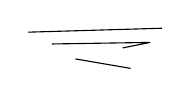
\begin{tikzpicture}\draw (0,0)--(1.7,.05);\draw (.3,-.15)--(1.55,-.13)--(1.2,-.2);\draw (.6,-.34)--(1.3,-.46);\end{tikzpicture}}
\figure{\begin{tikzpicture}\node[draw,ellipse] {V};\end{tikzpicture}}
\uline{\unsure{Relations|Relation} aux topologies} Supposons $R$ muni d'une topologie, donc les $R^I$ et les ``modèles'' modérés aussi. On voudrait que les applications modérées soient continues --- c'est OK si les parties modérées sont compactes (donc fermées, si $R$ séparé), c'est le cas. \deleted{Si le foncteur $X\mapsto$} \inserted{Supposons donc}
\figure{\begin{tikzpicture}\node[draw,ellipse] {$M9$};\end{tikzpicture}}
\[
 \left\{\begin{array}{l}R\text{ séparé}\\
 \text{les parties modérées de }R^n\text{ sont compactes}
 \end{array}\right.
\]
Alors le foncteur $X\unsure{-|\longrightarrow}|X|$ se factorise par la cat. des espaces topologiques
\[
 \operatorname{Esp}_{\mathcal M_*}\longrightarrow(\mathrm{Esp.\ top.\ cpts})
\]
\mspage{16}

\scanpage{18}
et ce foncteur est encore fidèle conservatif transportable \inserted{exact à gauche}. \deleted{\unsure{Je trouve}} On a une réciproque quand $R\in\deleted{\unsure{\operatorname{Esp}}}\mathcal M_1$ (donc $R$ cpt) en termes d'un tel foncteur et d'un objet $R\in\operatorname{Ob}\mathcal E$, tel que $\forall$ objet de $\mathcal E$ se plonge dans un $R^n$.

Tous espaces ind-modérés seront munis de la top. limite inductive. Elle induit sur chaque partie modérée sa topologie propre, quand on suppose que l'espace est ind-dénombrable, i.e. $\varinjlim$ de \uline{suites} croissantes d'espaces modérés.

On voudrait que dans un espace modéré, il y ait pour $\forall$ pt un syst. fond. de voisinages \deleted{de} modérés. Il suffit que \deleted{\unsure{ce}} \inserted{l'analogue} soit vrai dans $R$, donc dans les $R^n$, c'est l'axiome
\[
 (M10)\quad\text{Dans }R,\ \forall\text{ pt a un syst. fond. de voisinages}\in\mathcal M_1.
\]
\mspage{17}

\scanpage{19}
\mspage{9}
On voit \inserted{alors} que l'on a la notion d'application $X\longrightarrow Y$ entre espaces modérés, qui est \uline{modérée au voisinage d'un pt}, et on trouve

\uline{Prop} Pour qu'une application d'un espace modéré $X$ dans un espace ind-modéré soit modérée, il \unsure{faut s.} qu'elle le soit au voisinage de chaque pt.

Donc les applications modérées de $X$ dans $Y$ forment les sections d'un faisceau --- le faisceau des applications modérées de $X$ dans $Y$. La structure \inserted{modérée} de $X$ est connue quand on connaît l'ens des applications modérées de $X$ dans $R$ (cela \deleted{\unsure{faut}} dans le contexte purement ensembliste, avec $\unsure{(M1)_0|(M1)}$, $(M2)$ $(M3)$ $(M4)$ seulement), donc aussi quand on connaît le faisceau des germes de fonctions modérées.
\mspage{18}

\scanpage{20}
\uline{Espaces loc. modérés} Esp. \deleted{loc. cpts} \inserted{ind-modérés} dont la top. est \deleted{loc. cpt} séparée, et $\forall$ point admet un \uline{voisinage} qui est \deleted{\unsure{esp.}} modéré (donc l'espace est loc. cpt), et $\forall$ pt admet un syst. fond. de voisinages modérés, et les parties compactes sont les parties contenues dans une partie modérée --- qui forment donc un antifiltre cofinal à celui des parties compactes.

Par exemple, par $(M10)$ $R$ est un espace $\mathrm{loc}^{\mathrm t}$ modéré, donc les $R^I$ aussi.

Les espaces loc. modérés \deleted{$\unsure{f}\ \operatorname{Esp}_{\mathrm{loc},\mathcal M_*}$} forment une sous-catégorie pleine $\operatorname{Esp}_{\mathrm{loc},\mathcal M_*}$ de $\underrightarrow{\operatorname{Esp}}_{\mathcal M_*}$, stable par $\varprojlim$ finies.

\margin{Dire qu'une partie compacte et \deleted{\unsure{fermée}} d'un espace modéré est modérée.}
\margin{\deleted{\unsure{loc.}}}
\figure{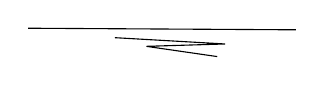
\begin{tikzpicture}\draw (0,0)--(3.4,-.02);\draw (1.1,-.12)--(2.5,-.2)--(1.5,-.23)--(2.4,-.36);\end{tikzpicture}}
\mspage{19}

\scanpage{21}
\mspage{20}\mspage{10}
\figure{\begin{tikzpicture}\node[draw,ellipse] {VI};\end{tikzpicture}}
\margin{\uline{Relation avec structure de corps}}
Oublions les structures topologiques, supposons par contre que $R$ ait une \uline{structure de corps}. On supposera alors, \deleted{\unsure{Alrt}} en plus de $(M1)_{\unsure{0}}$ et $(M4)$ (minimum pour construire $\operatorname{Esp}_{\mathcal M_*}$ avec ses $\varprojlim$ finies) l'axiome

\deleted{$(M11)$ \deleted{a) Pour $\forall$} partie modérée $A$ de $R$, l'application $a\mapsto-a$ de $A$ dans $R$ est modérée (i.e. l'ens $\{(a,-a)\in R^2\mid a\in A\}$ est \unsure{modéré})}

\figure{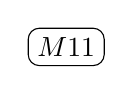
\begin{tikzpicture}\node[draw,rounded corners] {$M11$};\end{tikzpicture}}
a) $0$ et $1$ sont $\in R_0$ i.e. $\{0\},\{1\}\in\mathcal M_1$

b) $\forall A\in\mathcal M_2$, les fonctions
\[
 (x,y)\longmapsto x-y\qquad
 (x,y)\longmapsto xy
\]
\deleted{c) $\forall A\subset R^*$, $A\in\mathcal M_1$, $\exists B\in\mathcal M_1$ tel que $A^{-1}\subset B$}
\margin{\deleted{(\unsure{NB}\ \unsure{OPS|OB}\ $B\supset A^{-1}$)}}
sur $A$ sont modérées, \deleted{\unsure{car}} i.e. les deux parties de $R^3$
\[
 \{(x,y,x-y)\mid(x,y)\in A\},\qquad\text{et }\{(\unsure{x|a},y,xy)\mid(x,y)\in A\}
\]
sont modérées.

c) $\forall A\subset R^*$, $A\in\mathcal M_1$, $\exists B\in\mathcal M_1$ avec $A^{-1}\subset B$ \unsure{(OPS $B=A^{-1}$)}.

\deleted{\unsure{Et axiome}} \deleted{\unsure{les parties a) b)}} \inserted{les parties a) b)} équivalent à la validité de la

\margin{\uline{NB} Si $R\in\mathcal M_1$, il suffit de prendre $(M11)$ pour $A=R^2$}

\uline{Proposition} Pour un espace modéré $X$, les fonctions modérées $X\unsure{-|\longrightarrow}R$ \deleted{\unsure{est = un sous $R_0$}} forment un \uline{sous-anneau} de l'anneau des fonctions scalaires sur $X$. En particulier, $R_0$ est un sous-anneau de $R$, et les anneaux
\margin{de fonctions mod. \unsure{sont} des $R_0$-algèbres}

\scanpage{22}
De $=$ pour $X$ un espace ind-modéré, p.ex. (si $R$ est réunion de ses parties modérées $(M8)$ i.e. \inserted{les $R^I$} sont des espaces ind-modérés) pour les fonctions ind-modérées sur les $R^I$, qui contiennent en tous cas les \deleted{ensembles} anneaux de polynômes $R_0[(X_i)_{i\in I}]$ en les fonctions coordonnées.

\margin{Donc les applications $R_0$-polynomiales \deleted{\unsure{entre}} \deleted{\unsure{transfont}} $R^I$ sont modérées, et transfont des parties modérées en \unsure{itou}.}

\uline{Corollaire} Soit $f$ une fonction modérée sur l'espace modéré $X$. Alors $f$ est inv. \unsure{(dans|dans} l'anneau des fonctions modérées ssi $f$ ne s'annule pas dans $X$.

En considérant $f(X)\subset R^*$, cela revient au

\uline{Corollaire} Soit $A\subset R^*$, $A\in\mathcal M_1$, alors la restriction de $x\mapsto x^{-1}$ à $A$ est modérée, i.e. l'ens des $(x,x^{-1})\in R^2$, $x\in A$, est $\in\mathcal M_1$.
\mspage{21}

\scanpage{23}
\mspage{11}

En effet, c'est aussi l'ens des
\[
\{(x,y)\in R^2\mid xy=1,\ x\in A
\]
Si on suppose qu'il existe \deleted{$B\subset R^*$}, $B\in\mathcal M_1$, contenant l'ens \deleted{\unsure{des}} $\{x^{-1}\mid x\in A\}$, on \unsure{gagne}, car l'ens est la partie modérée de $A\times B$ image inverse de $1\in A.B$ \inserted{$=C\in\mathcal M_1$} par l'application modérée $(x,y)\mapsto xy$.

\uline{Cor} \uline{$R_0$ est un sous-corps de $R$}

\deleted{\unsure{Alors}}

Si $X$ modéré, $Y\subset X$ une partie modérée qui soit donnée comme dans M6 comme
\[
Y=\bigcap_{\alpha\in I} f_\alpha^{-1}(\{e_\alpha\})\qquad e_\alpha\in R,
\]
alors quitte à remplacer les $f_\alpha$ par $f_\alpha-e_\alpha$, \unsure{OPS} les $e_\alpha=0$, i.e. $Y$ est l'ens des \uline{zéros} communs à des $f_\alpha$.

Soient $(g_\beta)_{\beta\in J}$ \deleted{\unsure{des}} des fonctions \inserted{modérées} réalisant un plongement $X\subset R^J$. Considérons les $f_\alpha$, $f_\alpha g_\beta$ \deleted{\unsure{—}} elles sont toutes nulles sur $Y$, et

\mspage{22}

\scanpage{24}
\deleted{Si $x\in X\setminus Y$, $\exists\alpha$ tel que $f_\alpha(x)\ne0$, et}

définissent $Y$ comme l'ens des zéros communs. \deleted{de $X$} : ces fonctions, de plus elles séparent les pts de $X\setminus Y$, car si $x,y$ sont des pts distincts, \deleted{$\exists\beta$ tel que $f_\alpha(x)\ne0$ $g_\beta(x)\ne g_\beta(y)$ d'où}

Si les $f_\alpha$ \unsure{ne} suffisent pas à les séparer, montrons que les $f_\alpha g_\beta$ les séparent : en effet, $\exists\beta$ tel que $g_\beta(x)\ne g_\beta(y)$ \deleted{d'où} et $\alpha$ tel que $\lambda=f_\alpha(x)\ne0$, donc $f_\alpha(y)$ $(=f_\alpha(x)=\lambda\text{ par hyp.})\ne0$, d'où
\[
f_\alpha\underbrace{g_\beta(x)}_{\lambda}=\lambda g_\beta(x)\ne f_\alpha g_\beta(y)=\lambda g_\beta(y)
\]

Donc :

\uline{Proposition}. Si on a M1 à \unsure{M4} et M11, alors pour \unsure{$\forall$|tte} partie \deleted{\unsure{telle}} \inserted{modérée} $Y$ d'un esp. modéré $X$, qui est ens des zéros communs d'une famille finie de fonctions modérées sur $X$, on peut trouver une telle famille qui sépare les pts de $X$ (donc $X/Y$ est un espace modéré).

\mspage{23}

\scanpage{25}
À prouver

1) Si $X\to Y$ morphisme d'espaces modérés, $\exists$ partie modérée $Y'$ \uline{rare} dans $Y$ et
\[
(Z_i)_{i\in\underbrace{\pi_0(Y\setminus Y')}_{I}}=(U_i)_{i\in I},\quad Z_i\text{ modérés}
\]
\deleted{et des}
(de sorte que les $\unsure{\overline U_i|U_i}$ sont des parties modérées de $Y$) et enfin $\forall i\in I=\pi_0(Y\setminus Y')$, on ait une correspondance modérée
\[
R_i\subset(\overline U_i\times Z_i)\times X
\]
induisant une bijection entre $U_i\times Z_i$ et $X|U_i$ i.e. $X|\deleted{\unsure{(X\times_Y)}}U_i$ est fibré \deleted{\unsure{loc.}} trivial au sens modéré relatif ($U_i$ étant un espace modéré relatif \ldots)

Énoncé analogue pour un diagramme fini d'espaces modérés au dessus de $Y$ ?

Ce diagramme est \unsure{ess\textsuperscript{t}} ``trivial par morceaux'' au dessus d'un $Y\setminus Y'$ convenable, avec $Y'$ modéré rare dans $Y$ ??? Ce serait déjà intéressant dans le cas particulier \unsure{d'un} diagramme de la forme $Z\subset X\subset Y\times[0,1]$ \deleted{$\unsure{I\subset[0,}$} au dessus de $Y$\ldots

\mspage{24}
